\chapter{Datasets}
\label{chap:datasets} 

This appendix contains visualisations of the annotation for each dataset, as well as some representative images. The charts show a breakdown of; (a) categories of annotation derived from corrections applied, (b) types of user actions, (c) annotation rate in annotations per minute. All three charts use a gaussian density estimate with $\sigma=5 minutes$. 

The \emph{penguin survey} charts are split into it's three parts (each part was annotated separately).

\newpage
\section{penguins}

\begin{figure*}[!h]
\centering
  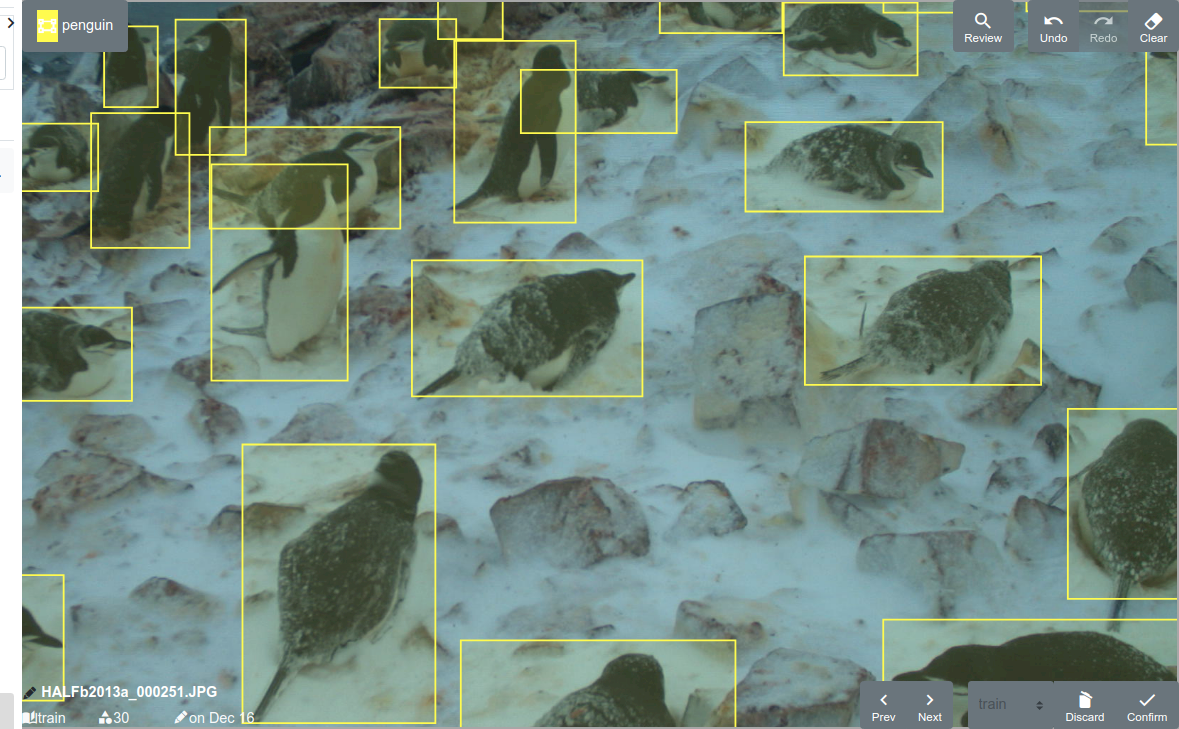
\includegraphics[width=0.475\linewidth]{figures/annotation/screenshots/penguins.png}
  \hfill
  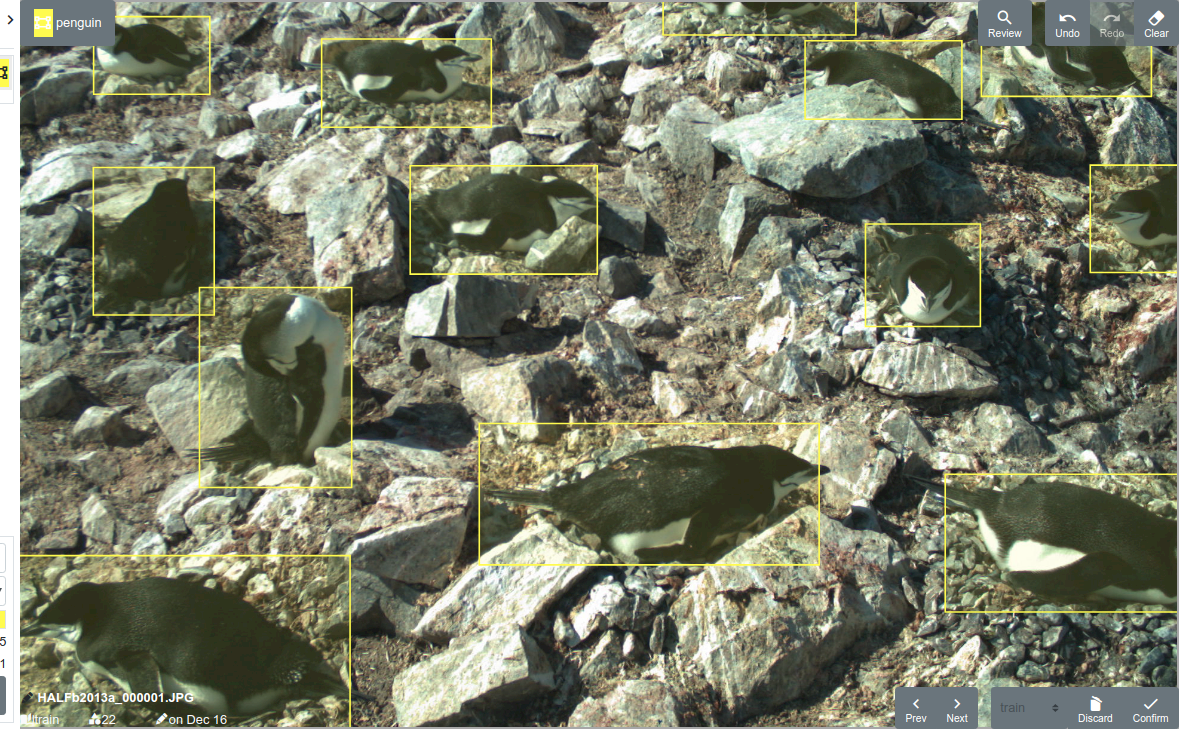
\includegraphics[width=0.475\linewidth]{figures/annotation/screenshots/penguins2.png}

\caption{Example images from the \emph{Penguin} dataset, \cite{PenguinData}}
\label{fig:penguin_dataset}
\end{figure*}

\begin{figure}[!h]
\centering
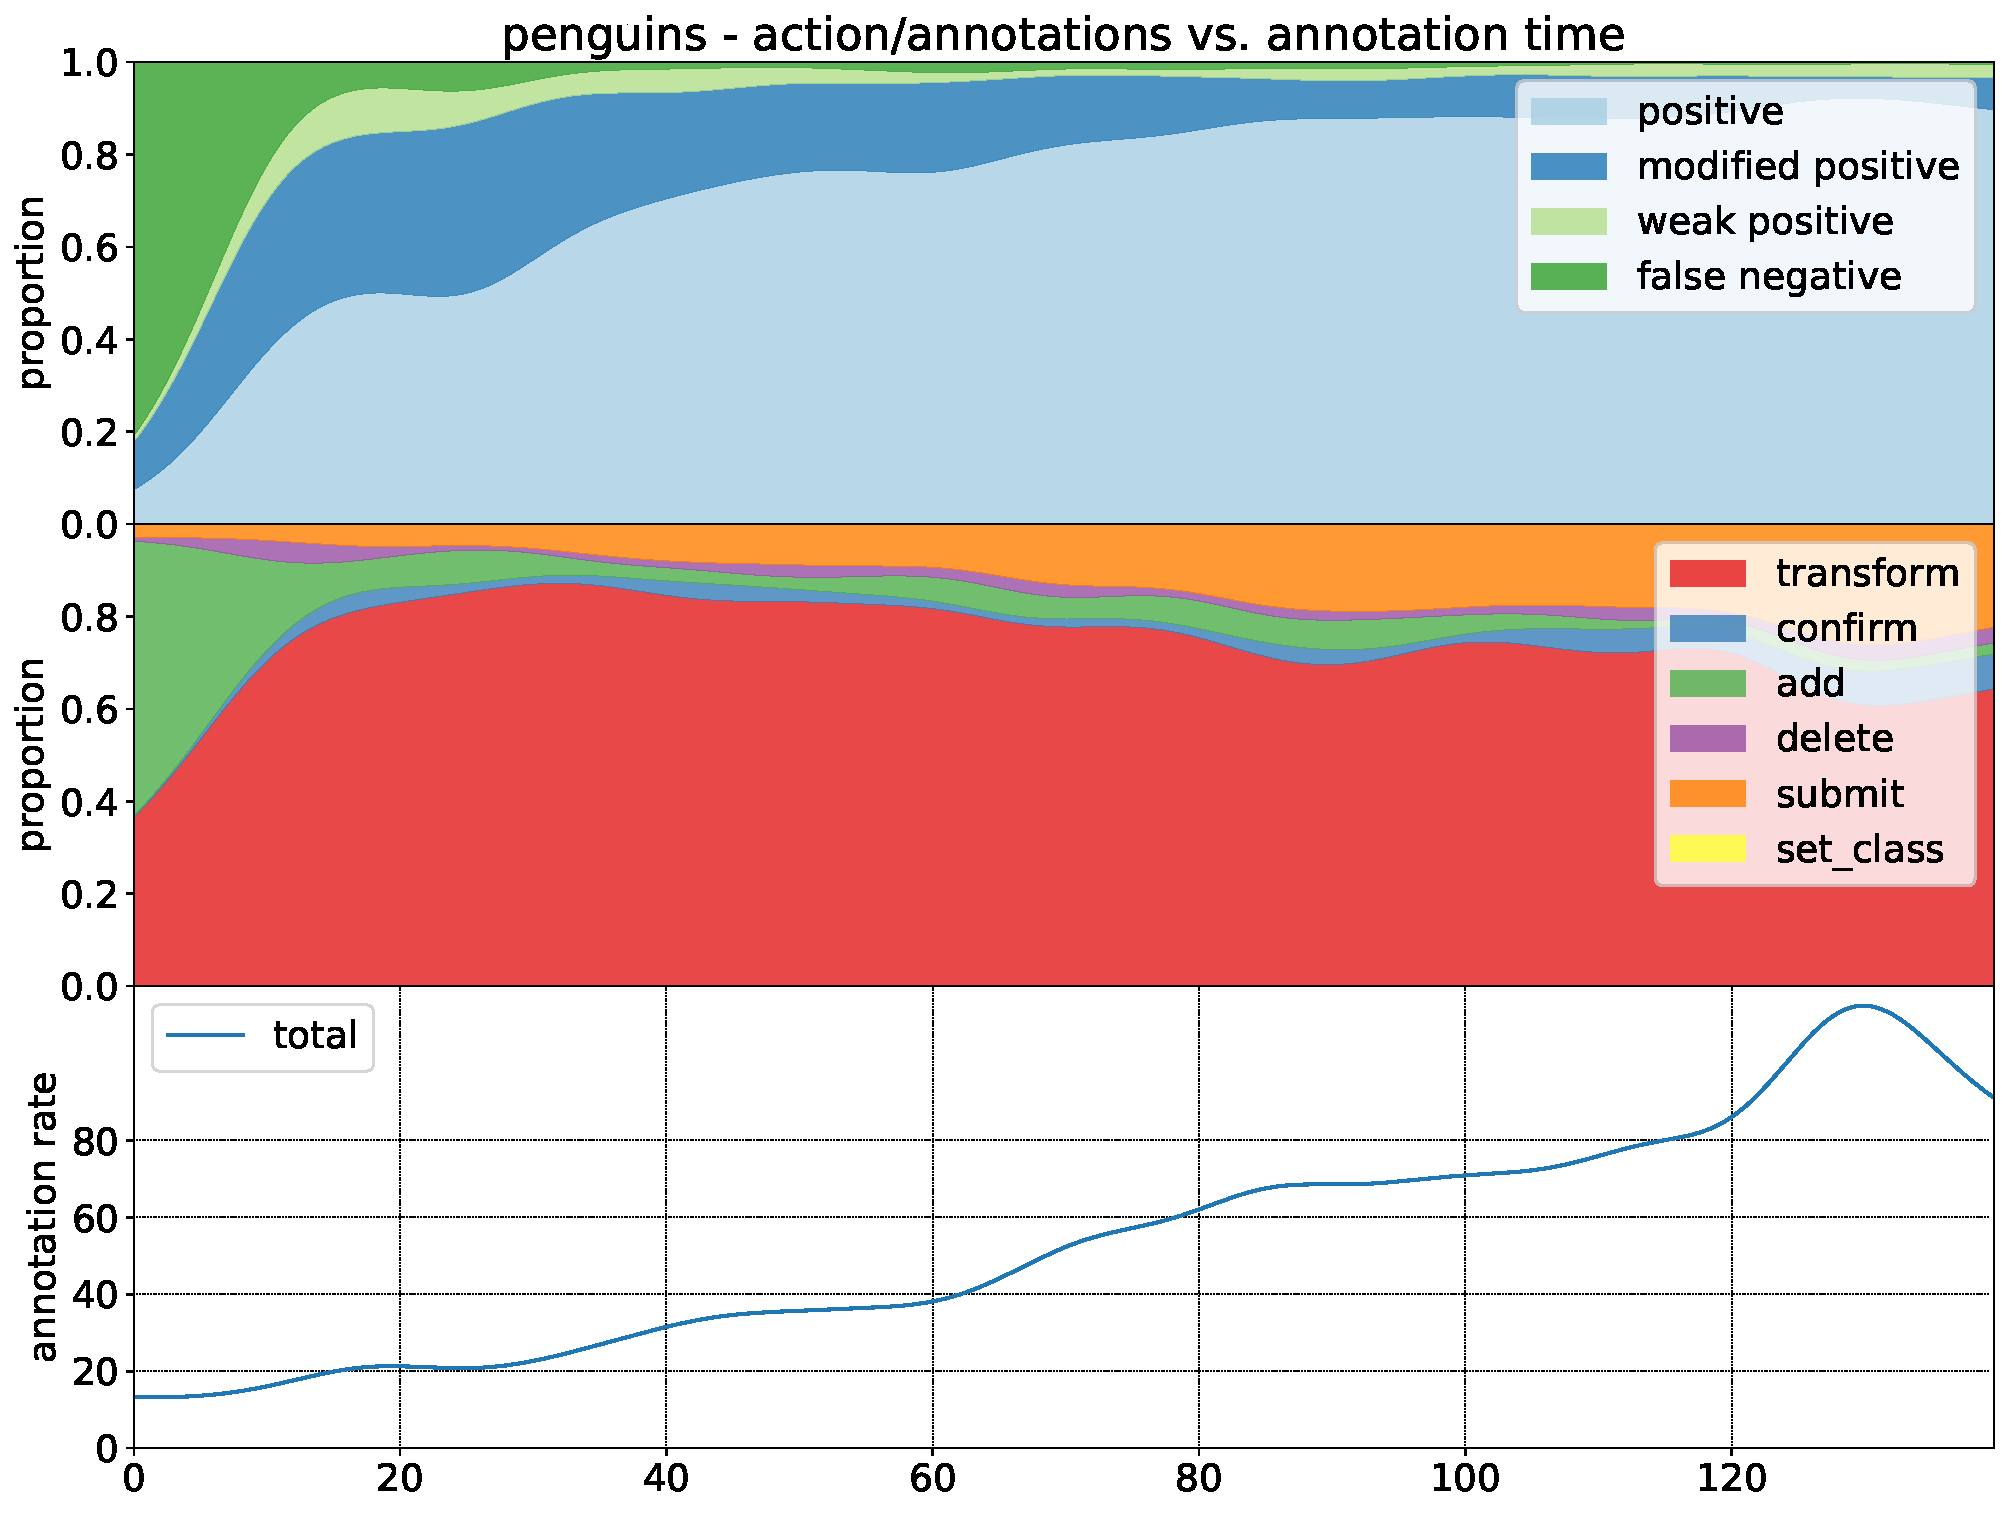
\includegraphics[width=1.0\linewidth]{charts/action_annotations/penguins.pdf}
\caption{  }
\label{fig:penguin_annotation}
\end{figure}



\pagebreak
\section{$\mathbf{apples^1}$}

\begin{figure*}[!h]
  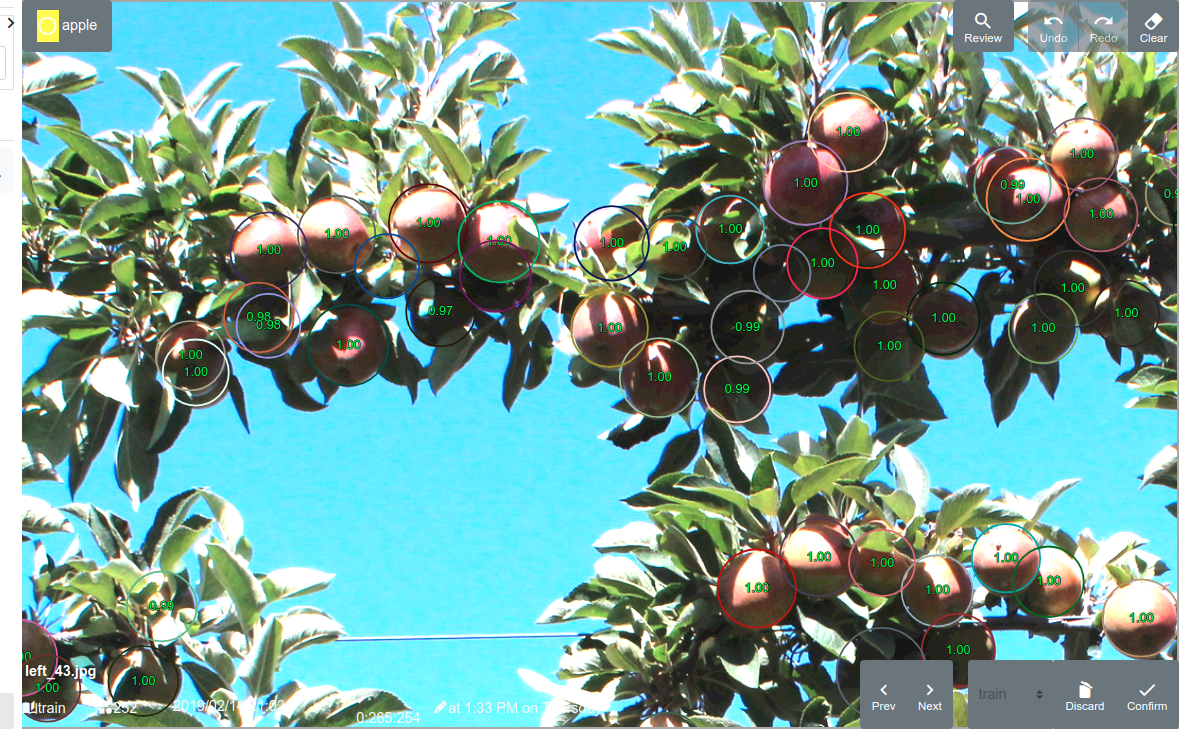
\includegraphics[width=0.475\linewidth]{figures/annotation/screenshots/apples_big.png}
  \hfill
  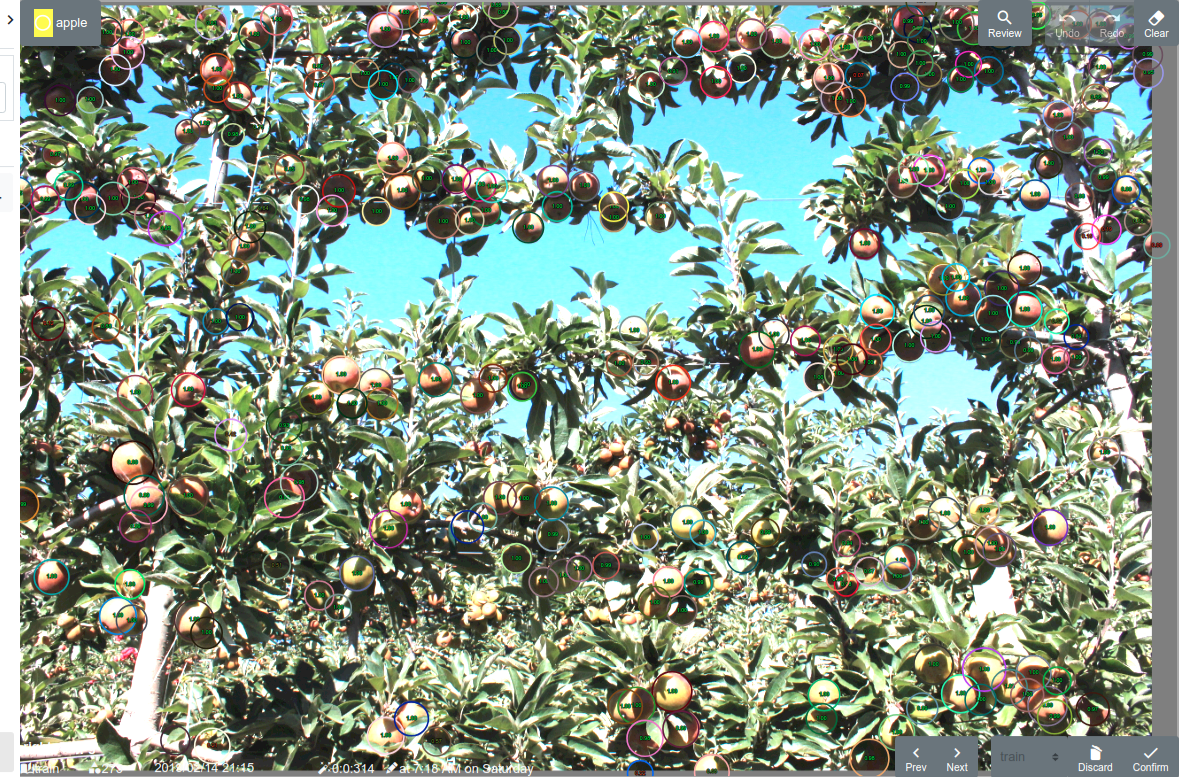
\includegraphics[width=0.45\linewidth]{figures/annotation/screenshots/apples_small.png}
\caption{Example images from the \emph{apples1} dataset}
\label{fig:apples1_dataset}  
\end{figure*}

\begin{figure}[!h]
\centering
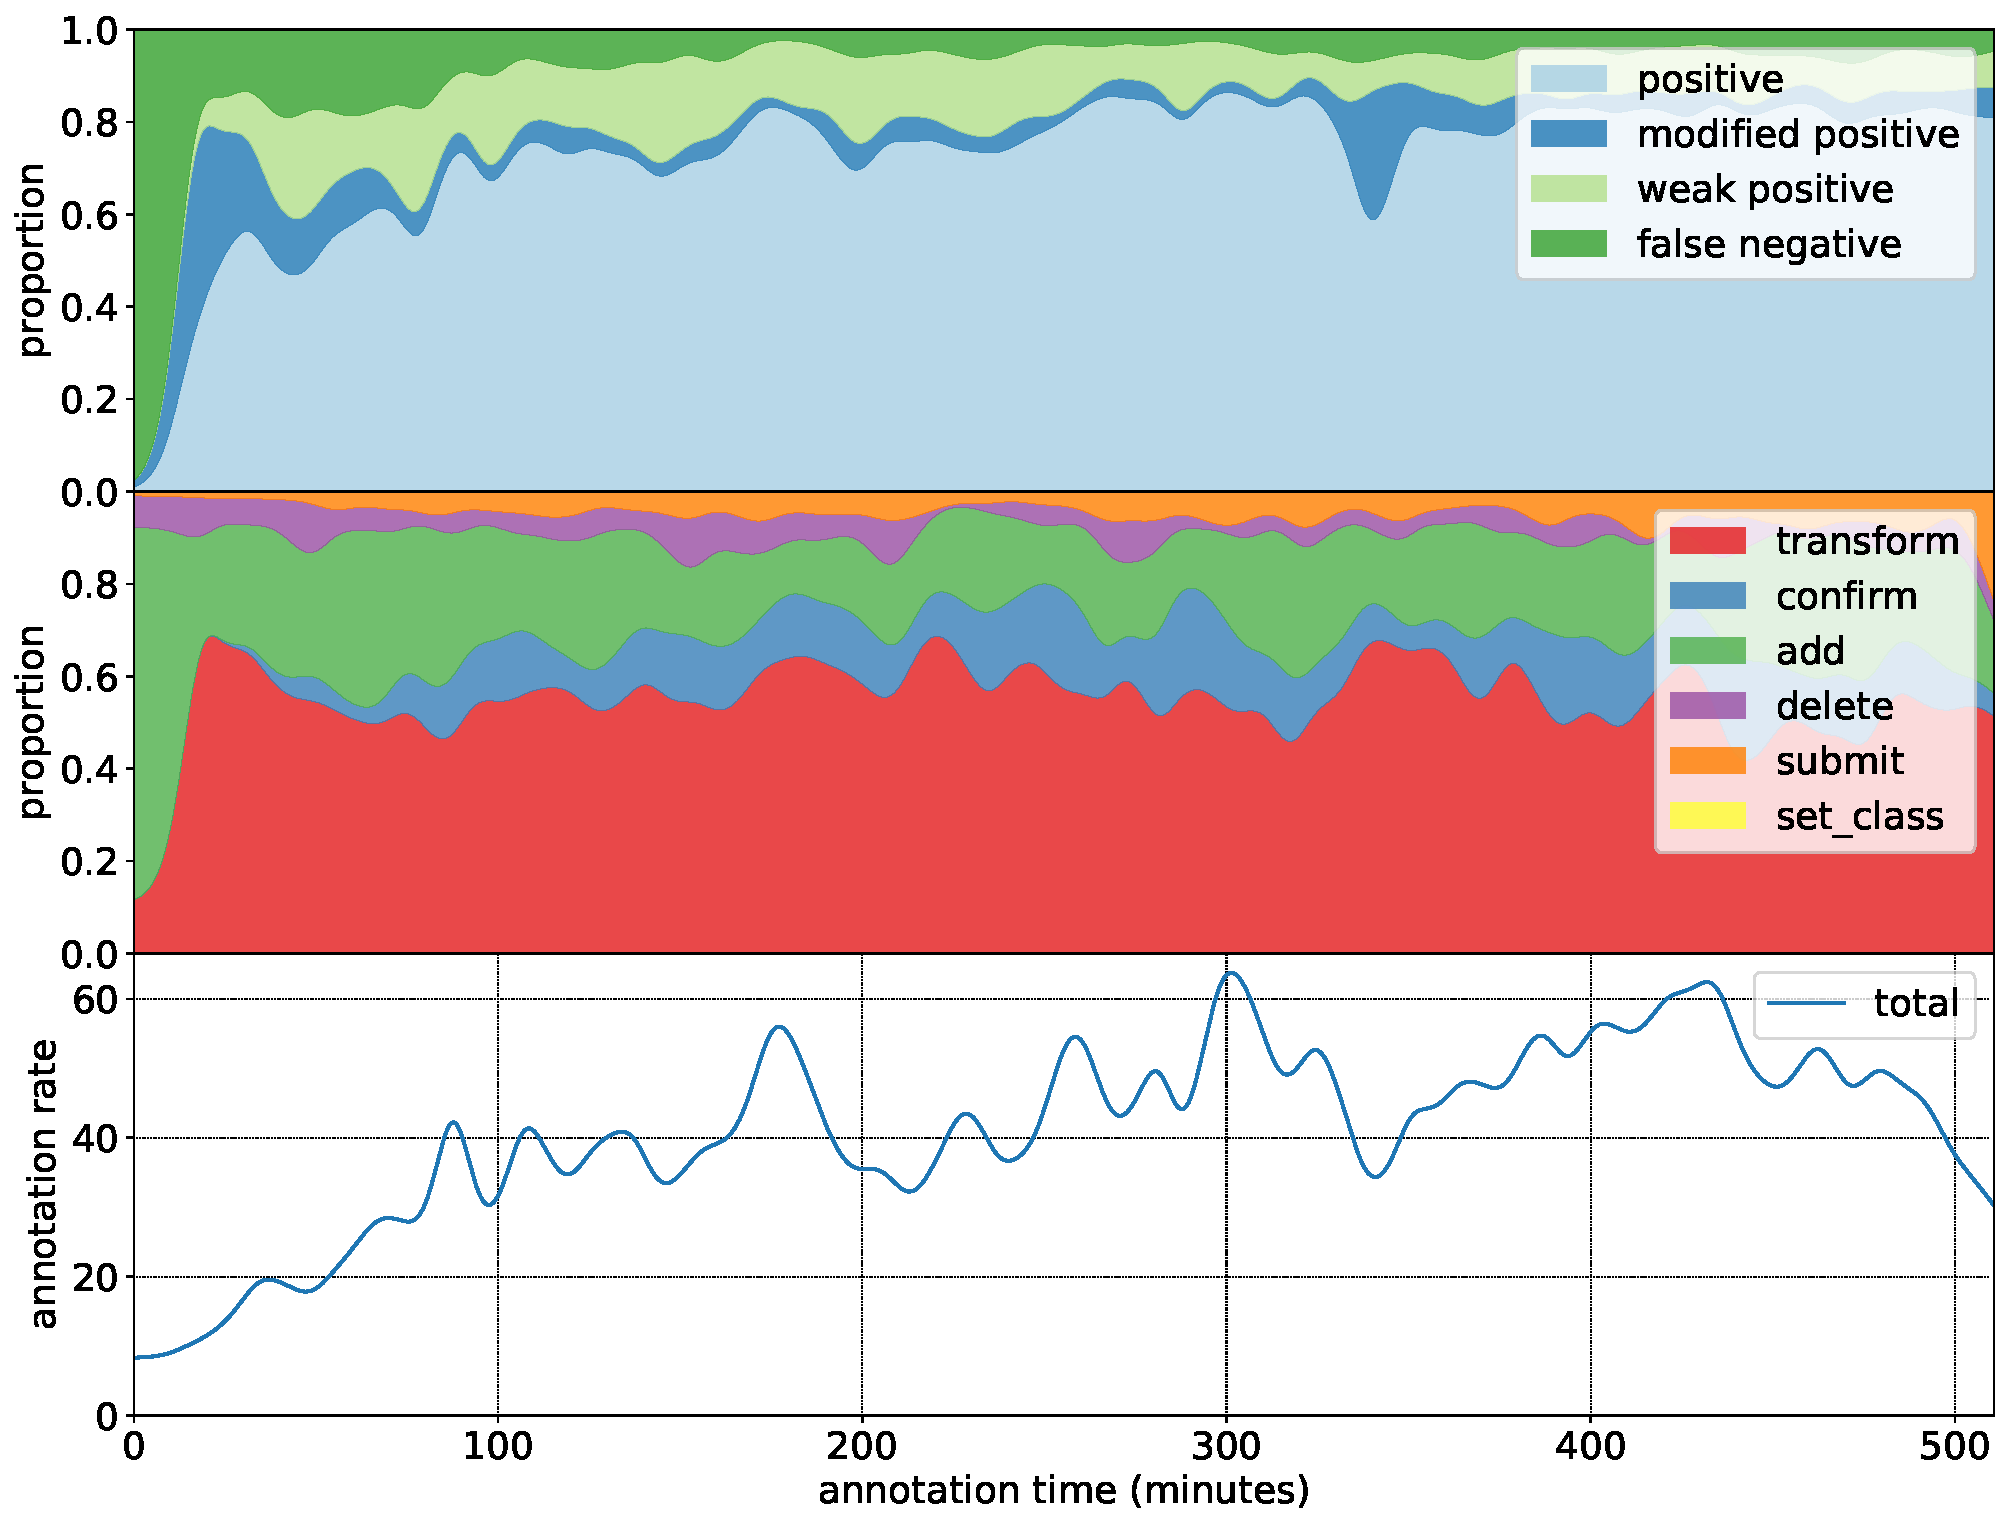
\includegraphics[width=1.0\linewidth]{charts/action_annotations/apples1.pdf}
\caption{  }
\label{fig:apples1_annotation}
\end{figure}

\pagebreak
\section{$\mathbf{apples^2}$}


\begin{figure*}[!h]
  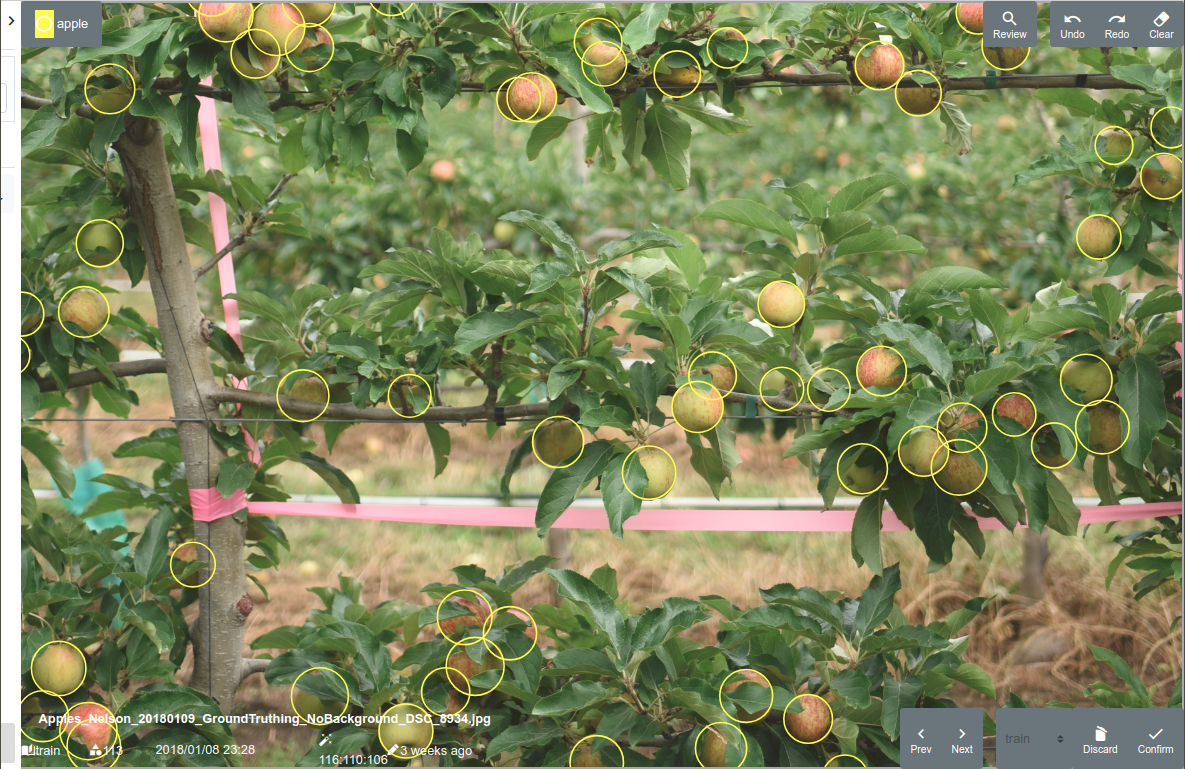
\includegraphics[width=0.475\linewidth]{figures/annotation/screenshots/apples2.png}
  \hfill
  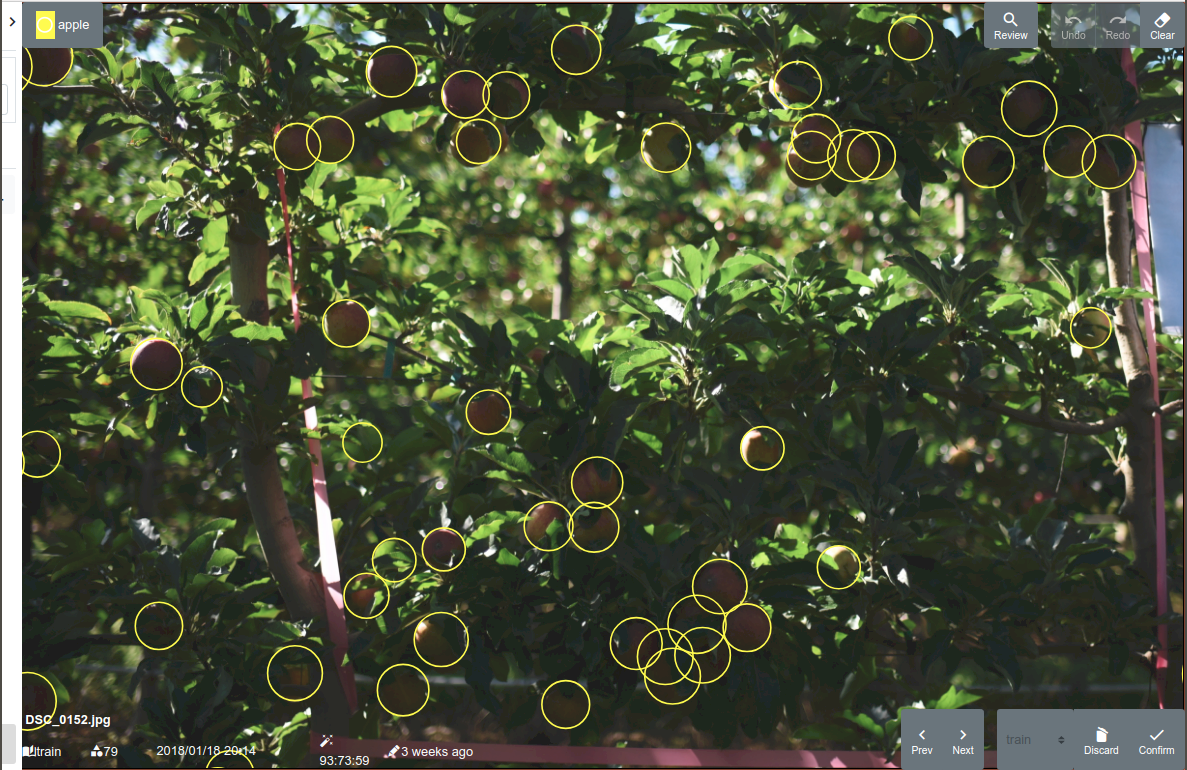
\includegraphics[width=0.475\linewidth]{figures/annotation/screenshots/apples2_dark.png}
\caption{Example images from the \emph{apples1} and \emph{apples2} datasets}
\label{fig:apples2_dataset}  
\end{figure*}

\begin{figure}[!h]
\centering
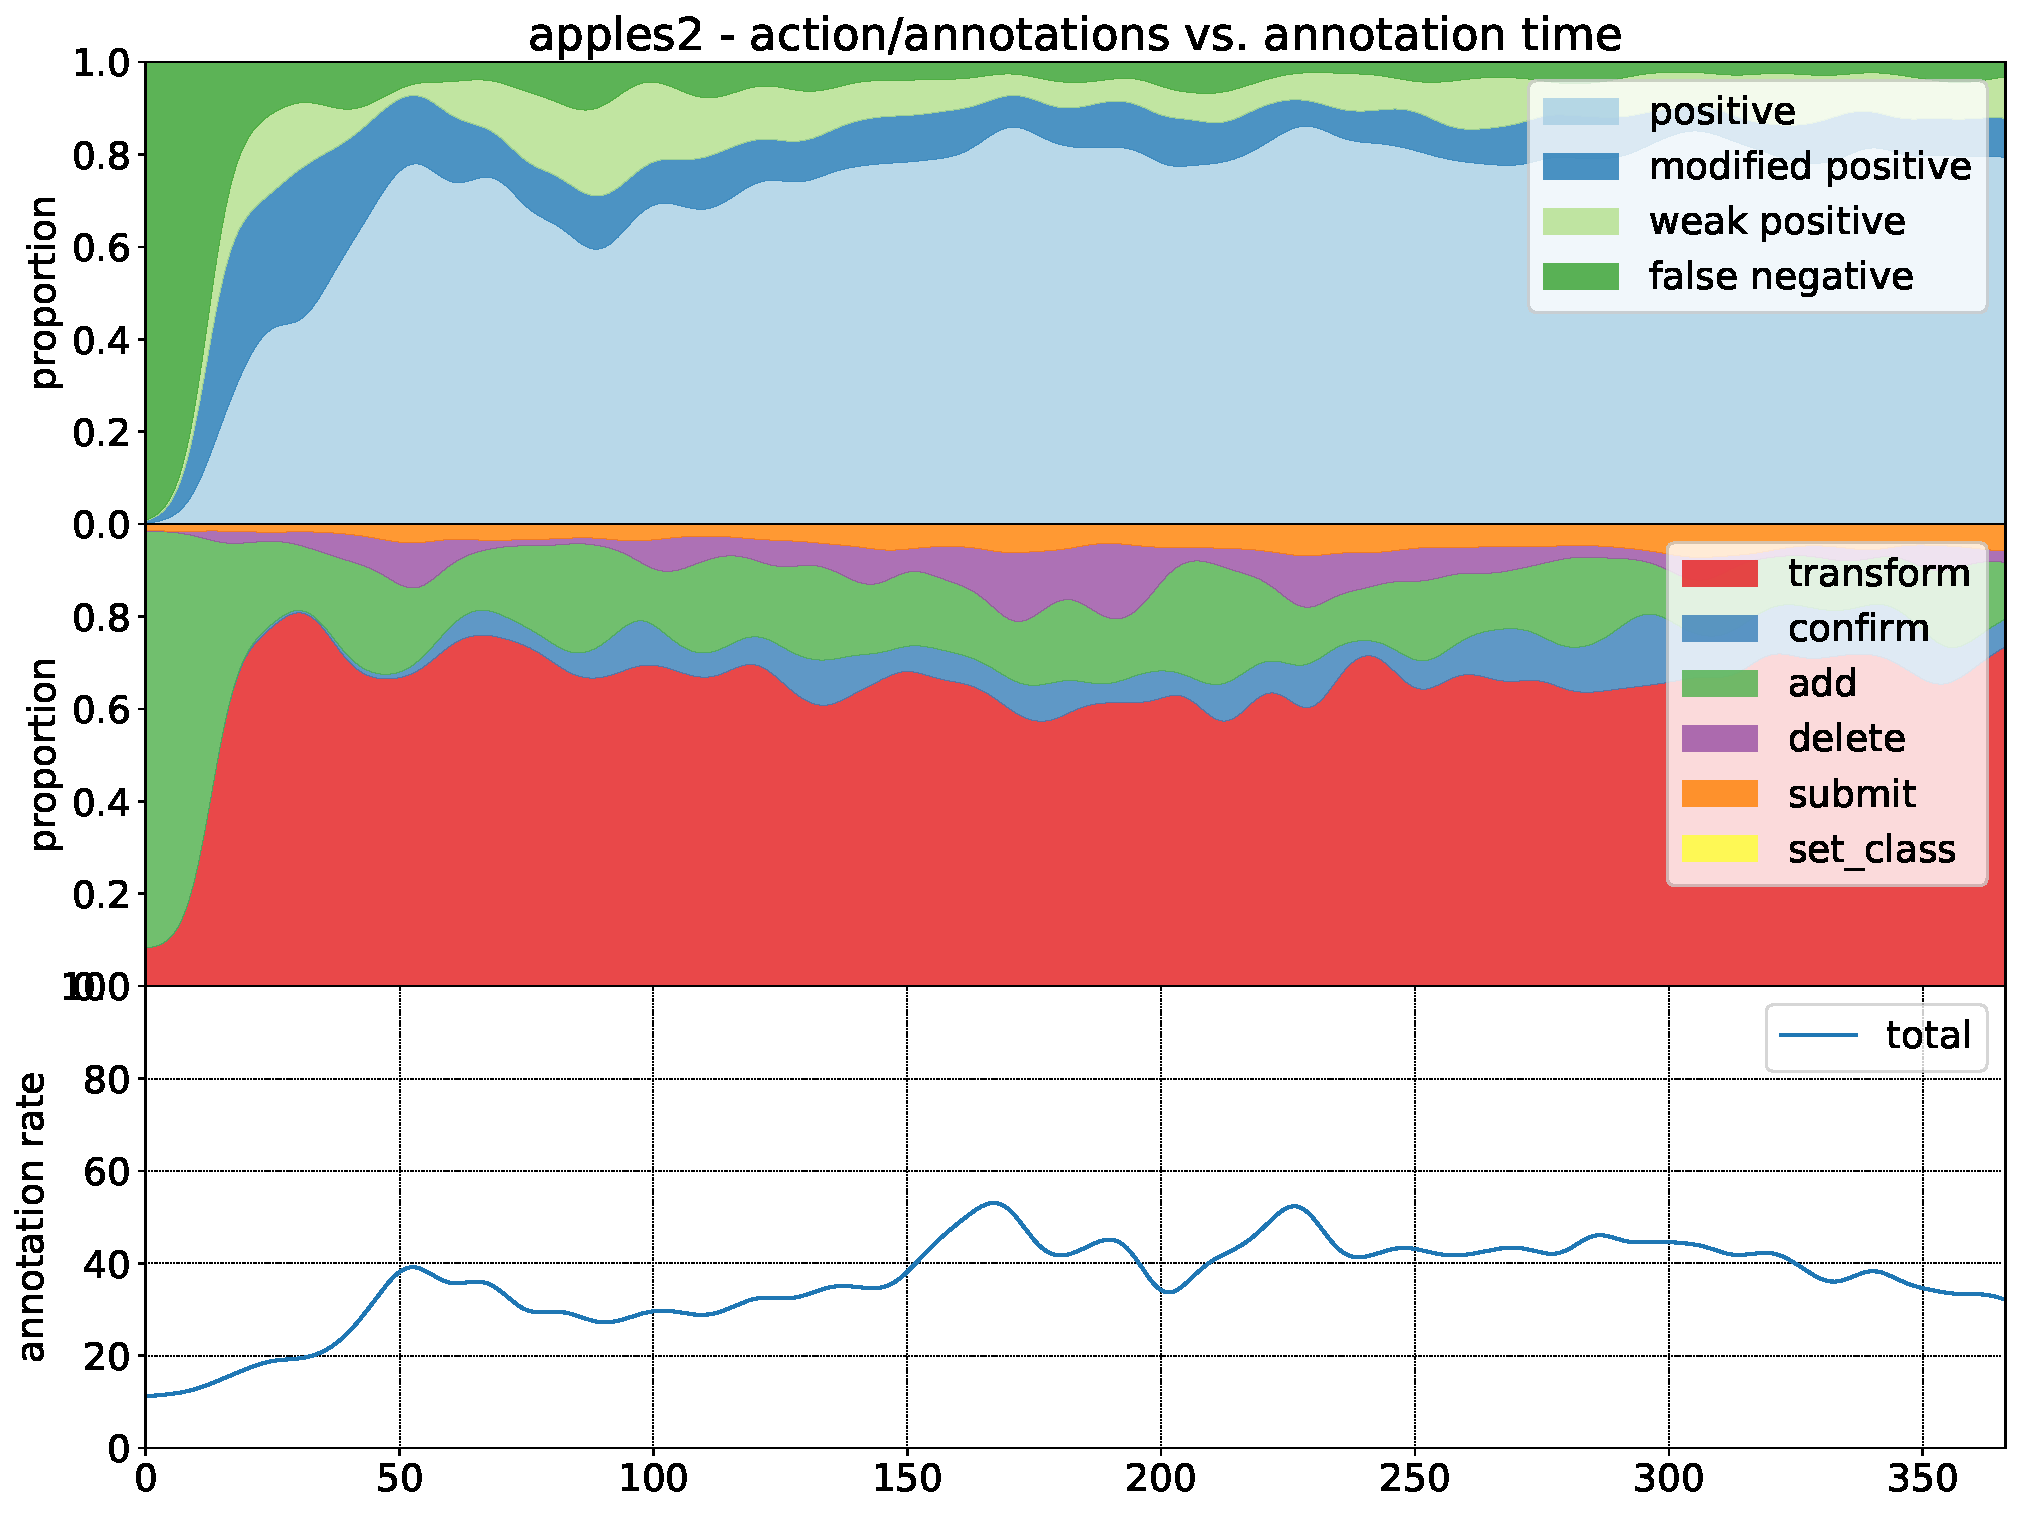
\includegraphics[width=1.0\linewidth]{charts/action_annotations/apples2.pdf}
\caption{  }
\label{fig:apples2_annotation}
\end{figure}

\pagebreak
\section{buoys}

\begin{figure}[H]
  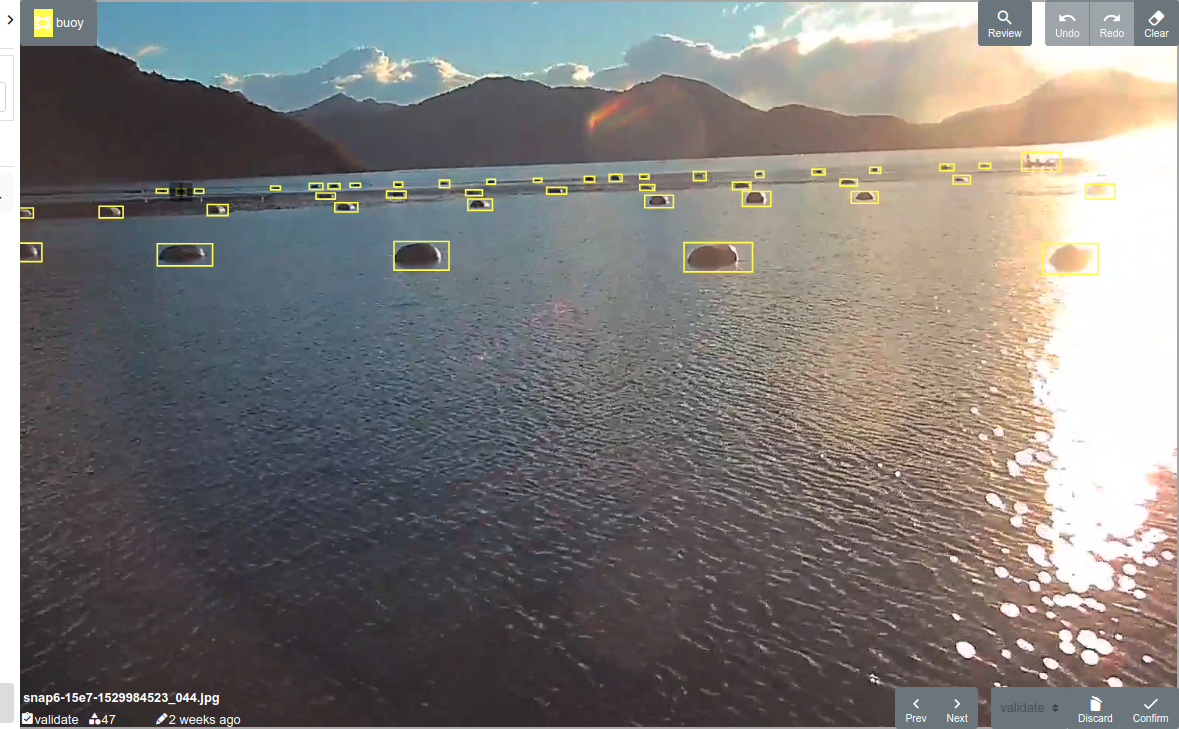
\includegraphics[width=0.475\textwidth]{figures/annotation/screenshots/buoys.png}
  \hfill
  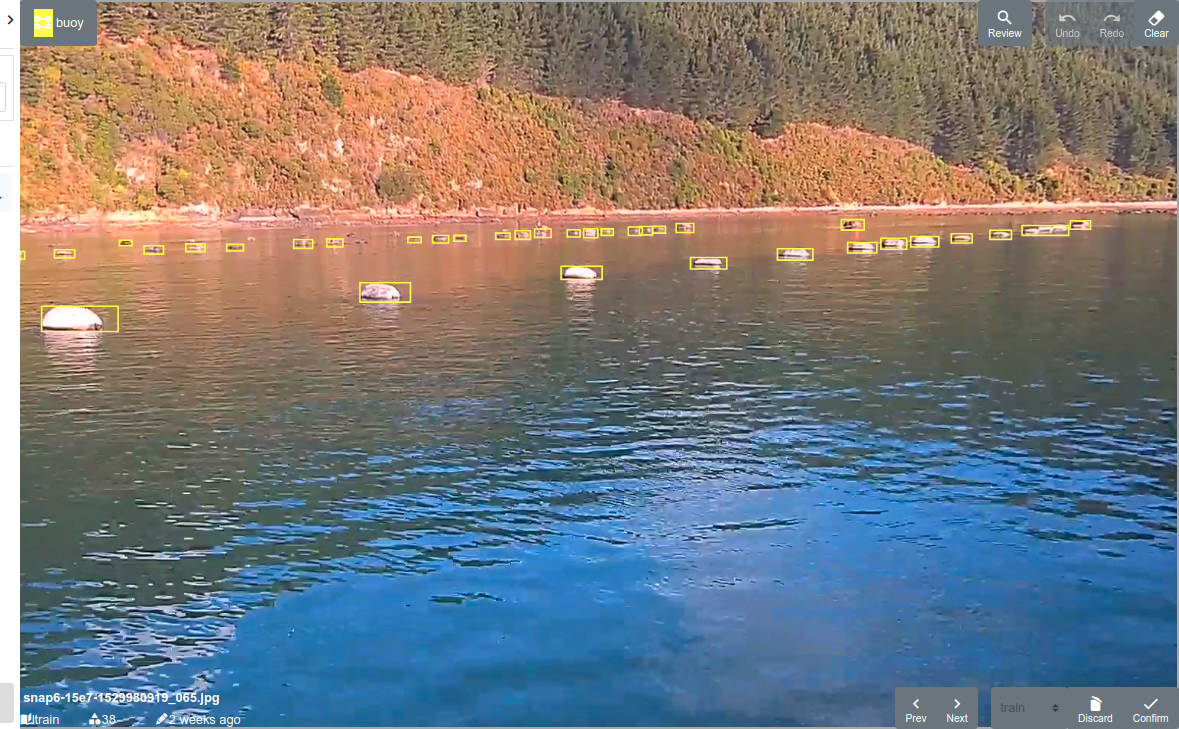
\includegraphics[width=0.475\textwidth]{figures/annotation/screenshots/buoys2.png}
  \caption{Example images from the \emph{buoys} dataset of mussel farm buoys captured from a camera attached to another buoy }
  \label{fig:buoys_dataset}
\end{figure}

\begin{figure}[!h]
\centering
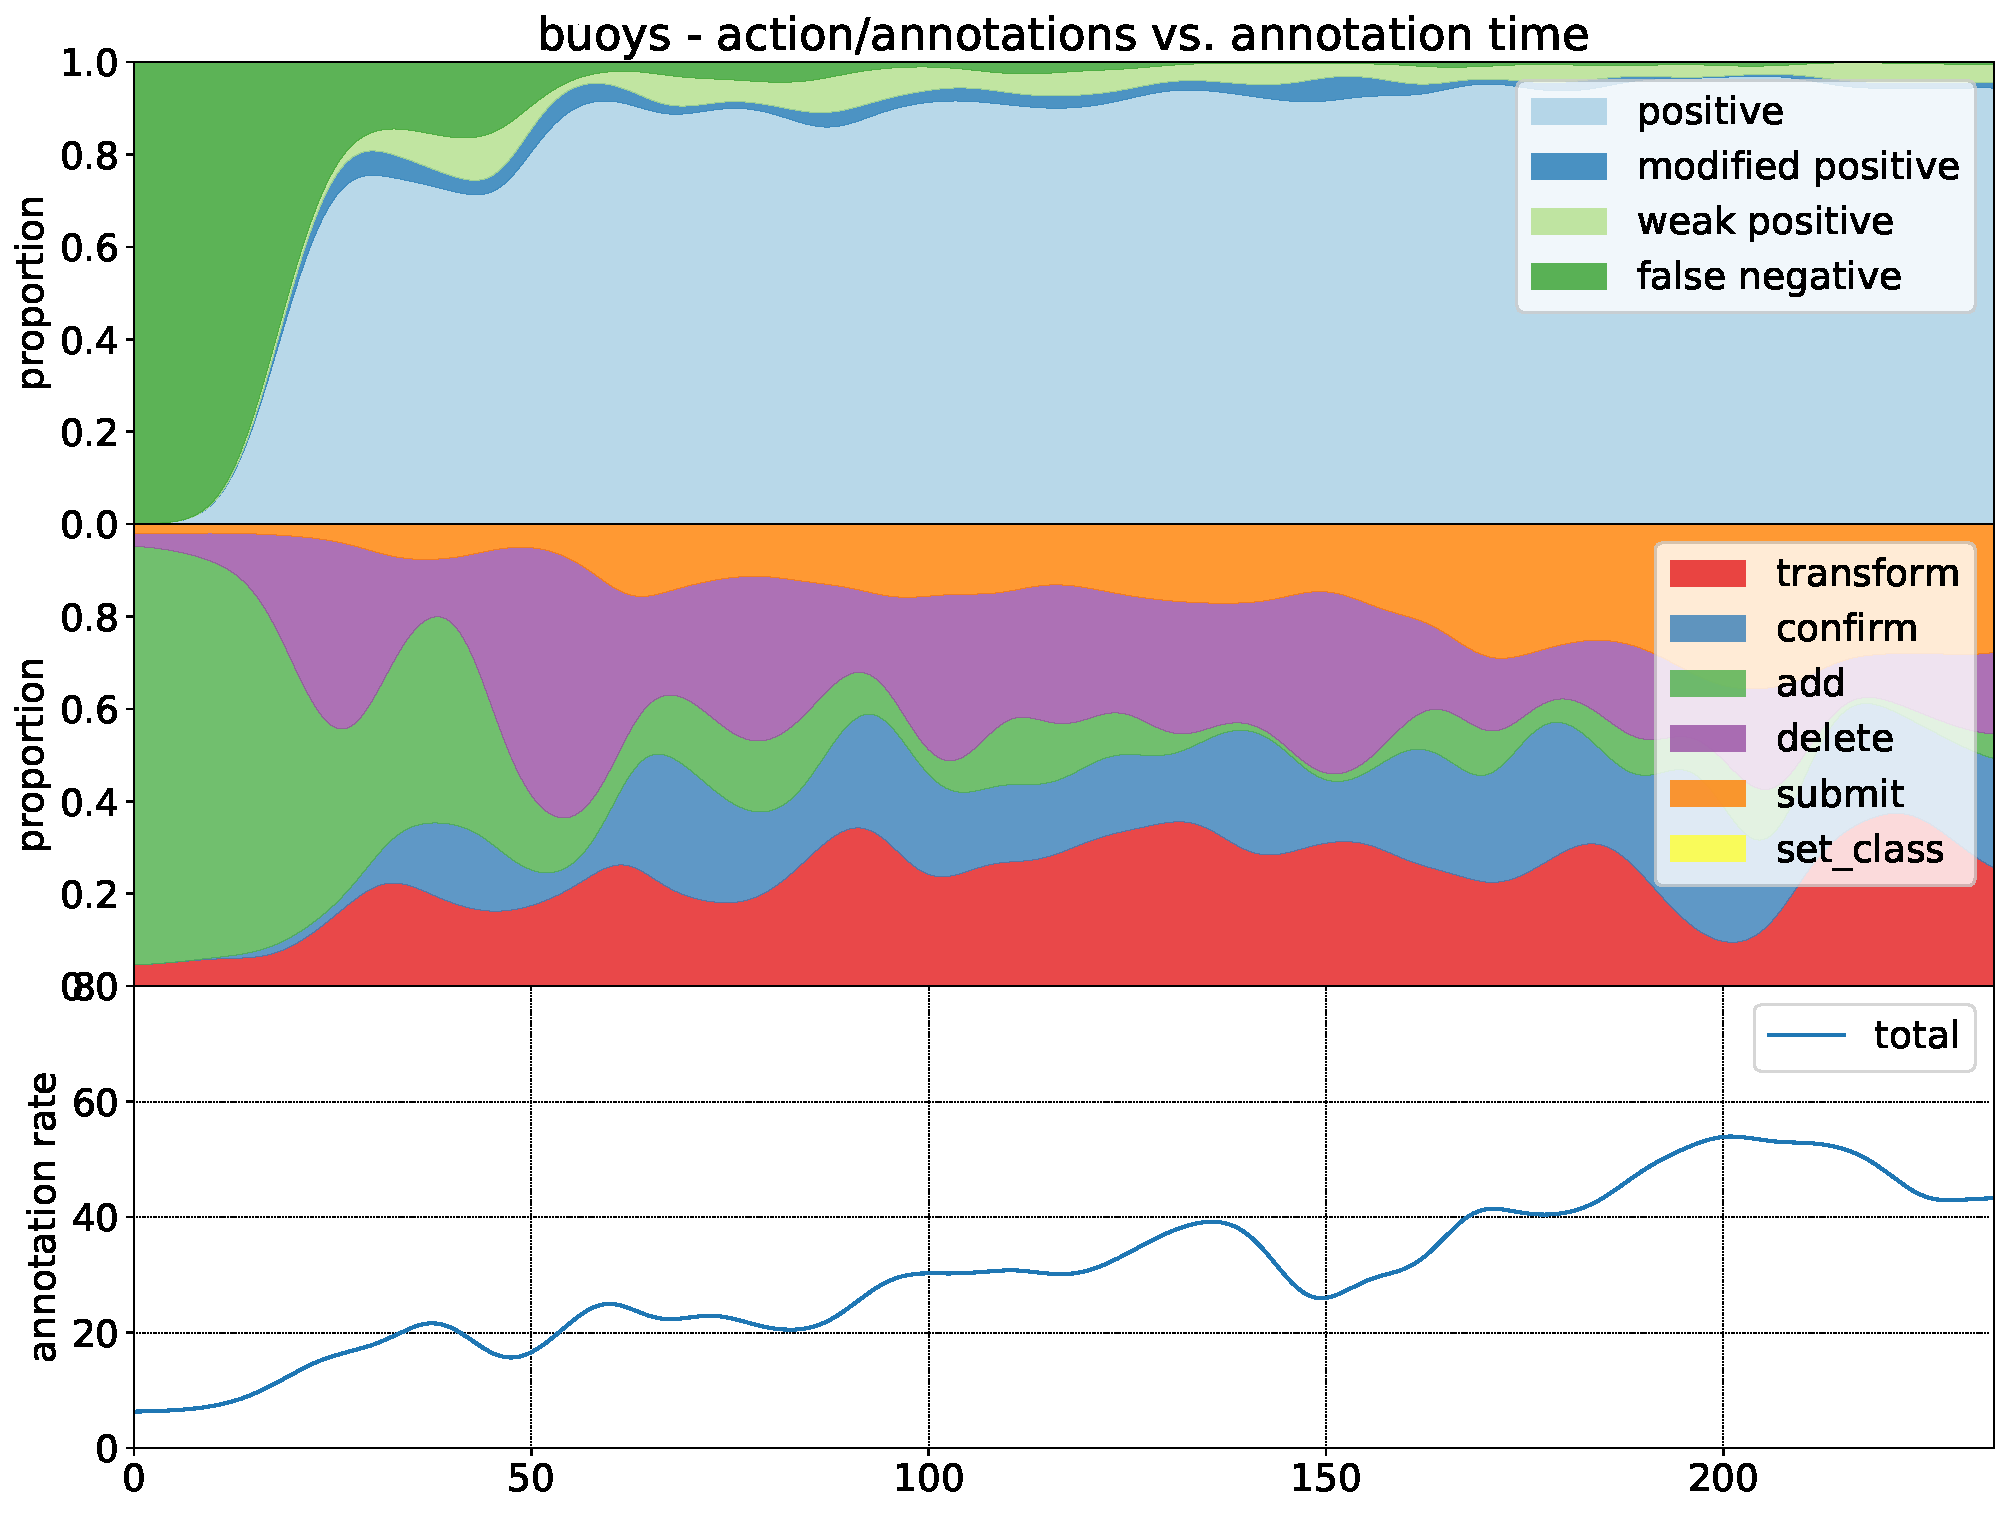
\includegraphics[width=1.0\linewidth]{charts/action_annotations/buoys.pdf}
\caption{  }
\label{fig:buoys_annotation}
\end{figure}

\pagebreak
\section{fisheye}

\begin{figure}[H]
\begin{center}
  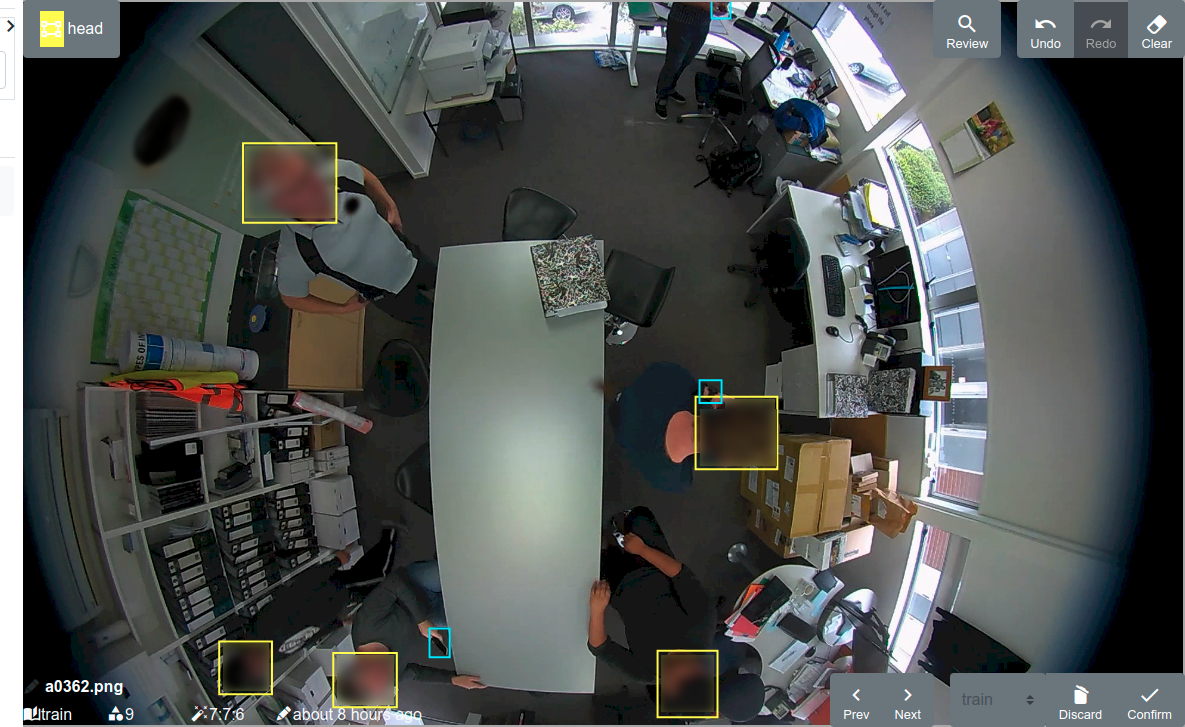
\includegraphics[width=0.5\textwidth]{figures/annotation/screenshots/victor.png}
\end{center}
  \caption{Example image from the \emph{fisheye} dataset of fish-eye lens head and cellphone detection }
\end{figure}

\begin{figure}[!h]
\centering
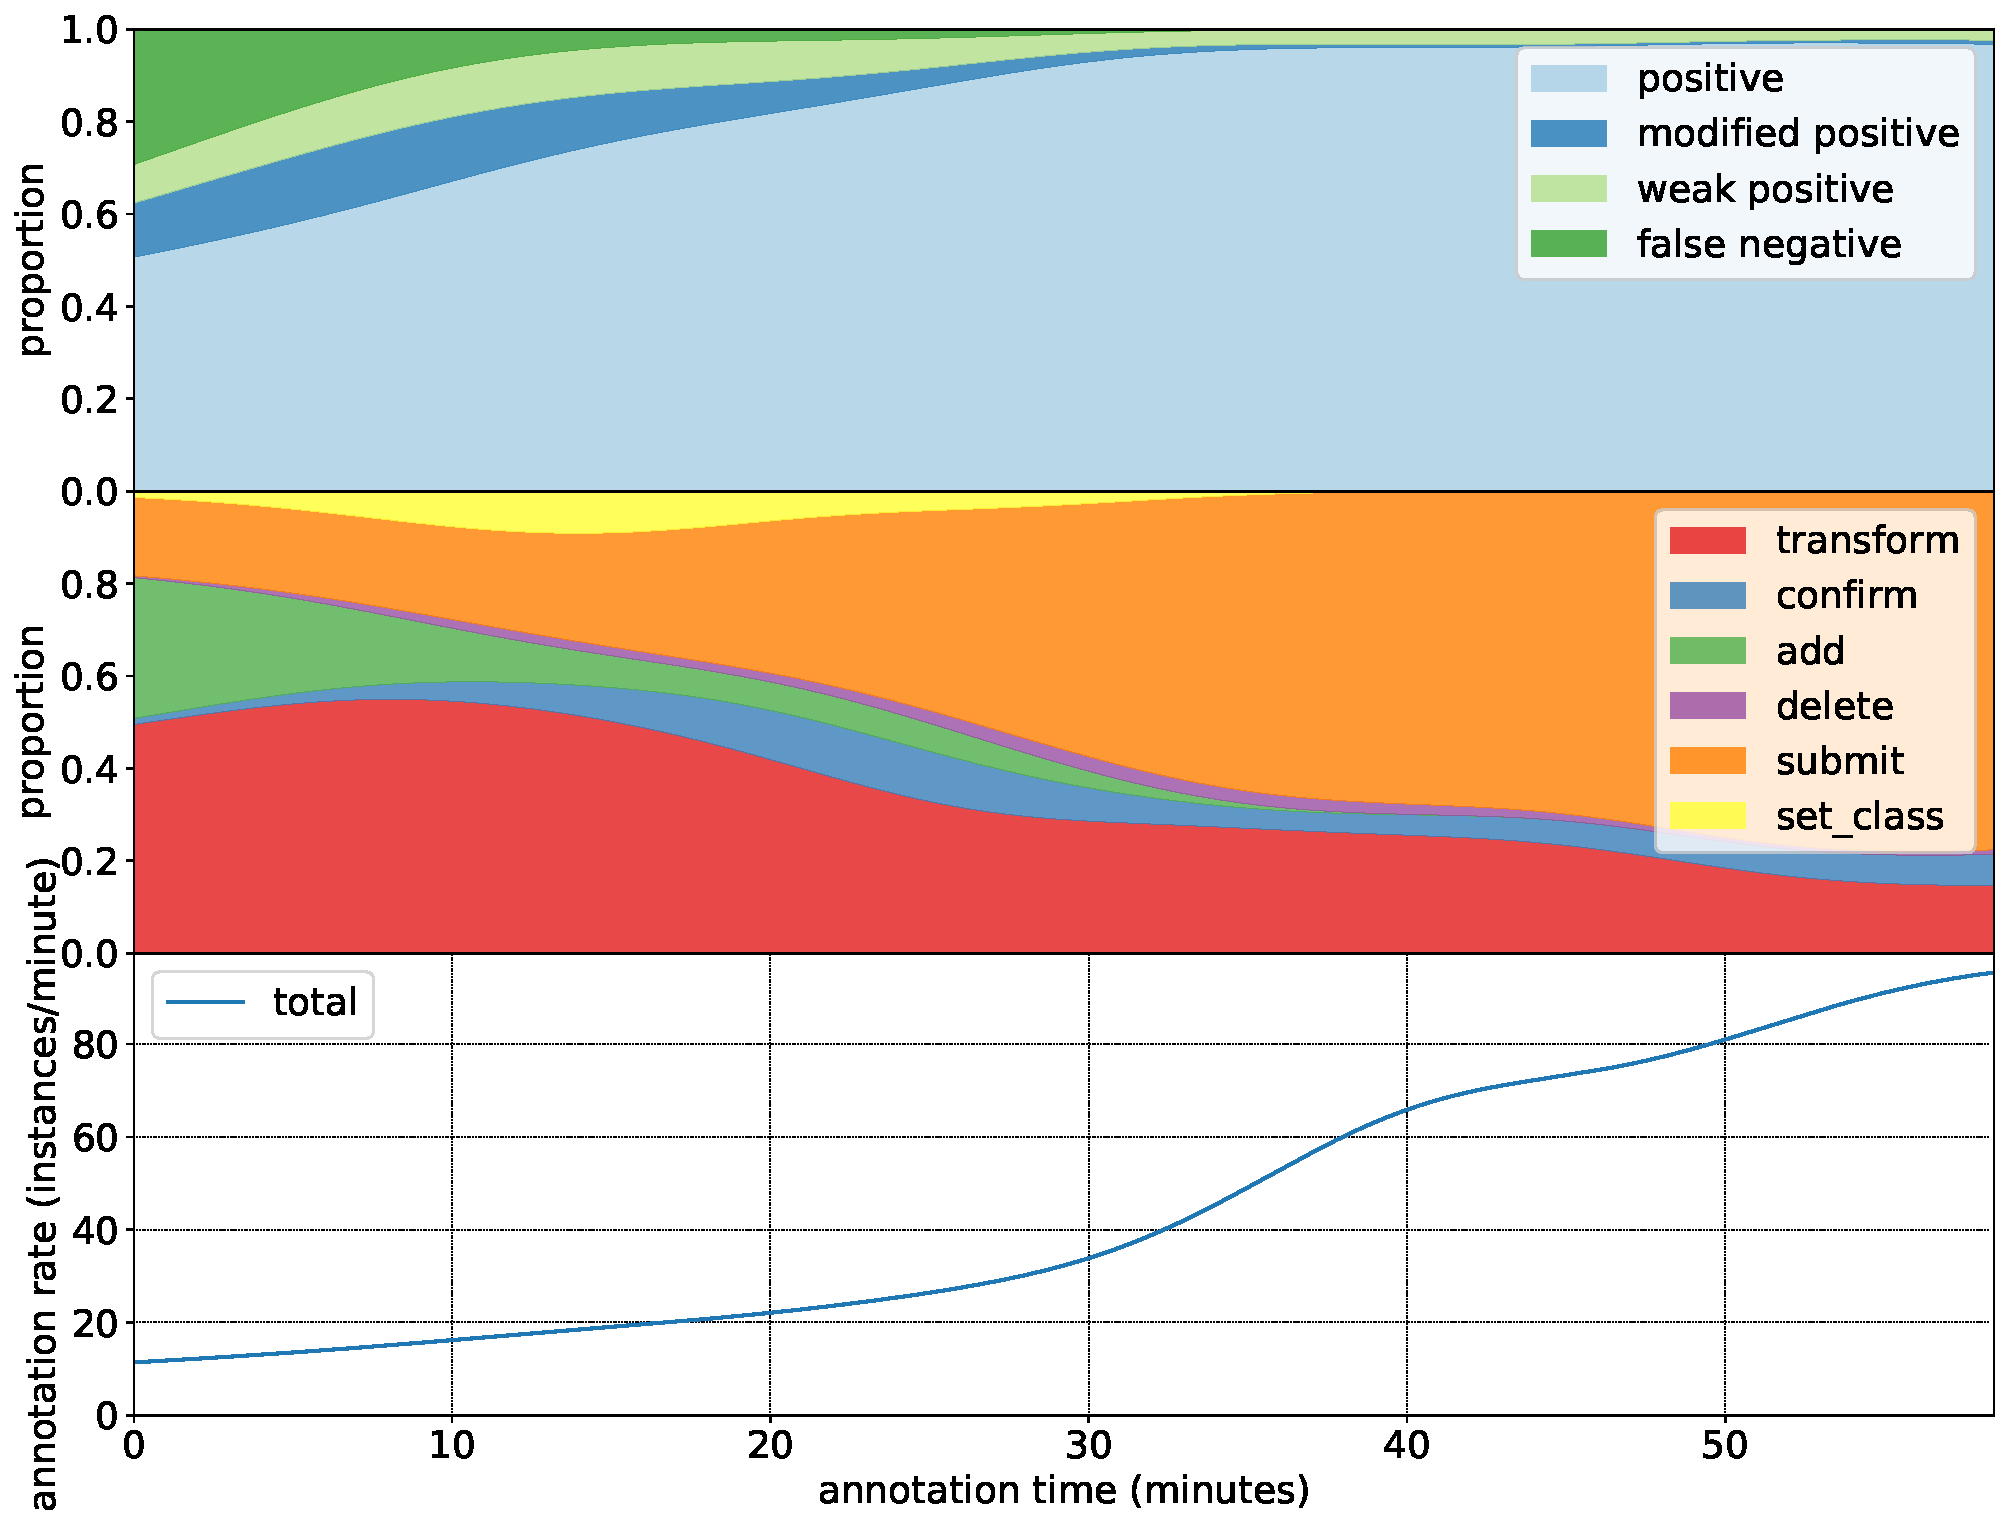
\includegraphics[width=1.0\linewidth]{charts/action_annotations/fisheye.pdf}
\caption{  }
\label{fig:fisheye_annotation}
\end{figure}


\pagebreak
\section{\emph{branches}}


\begin{figure}[!h]
  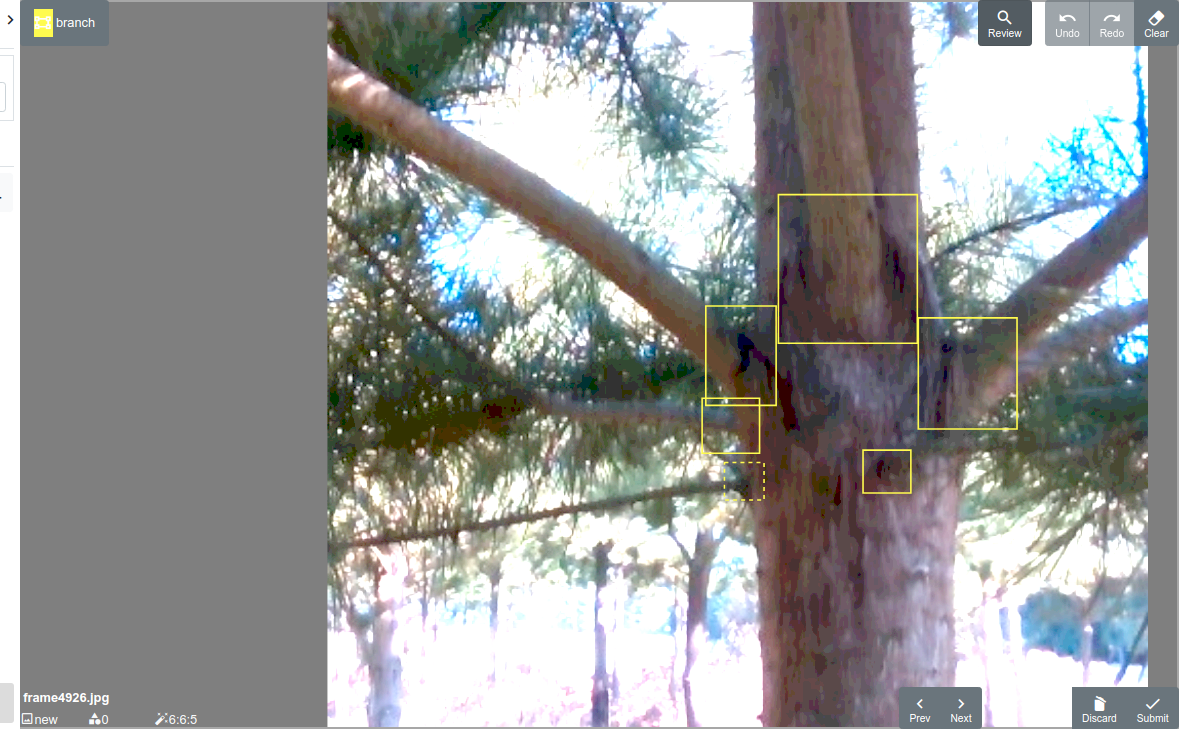
\includegraphics[width=0.475\textwidth]{figures/annotation/screenshots/branches3.png}
  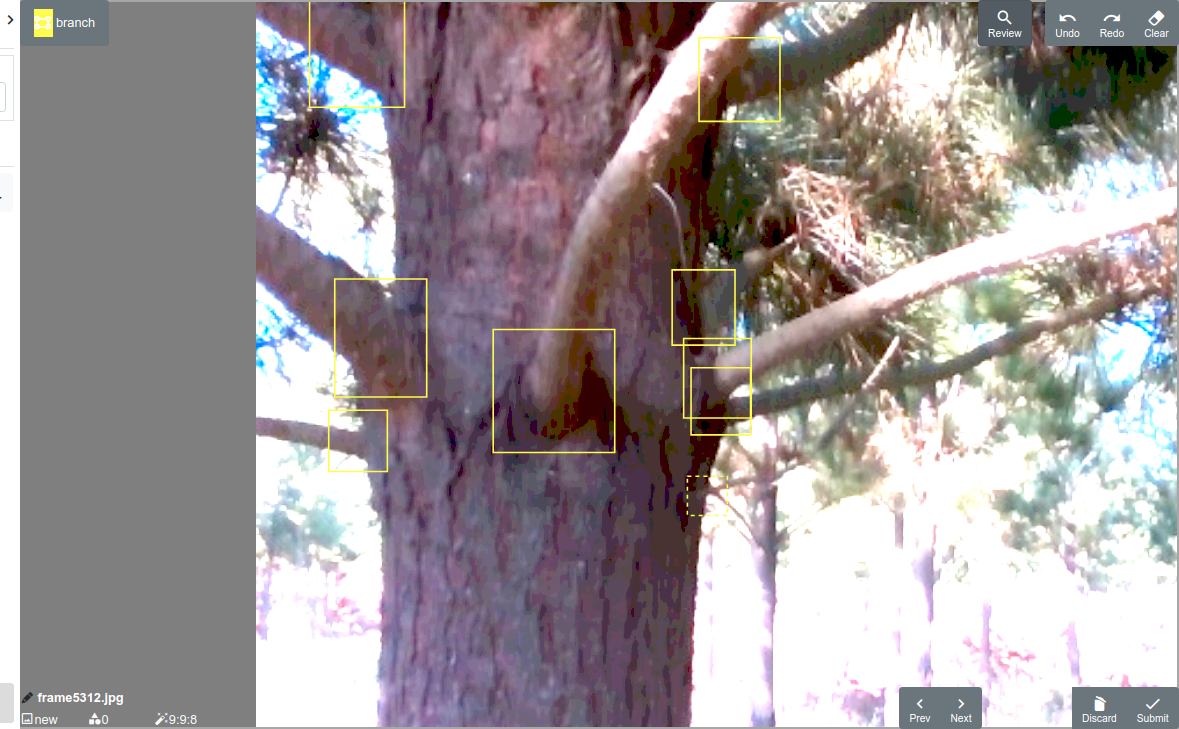
\includegraphics[width=0.475\textwidth]{figures/annotation/screenshots/branches2.png}  
  
  \caption{Example images from \emph{branches}, tree branch intersection detection}
\end{figure}

\begin{figure}[!h]
\centering
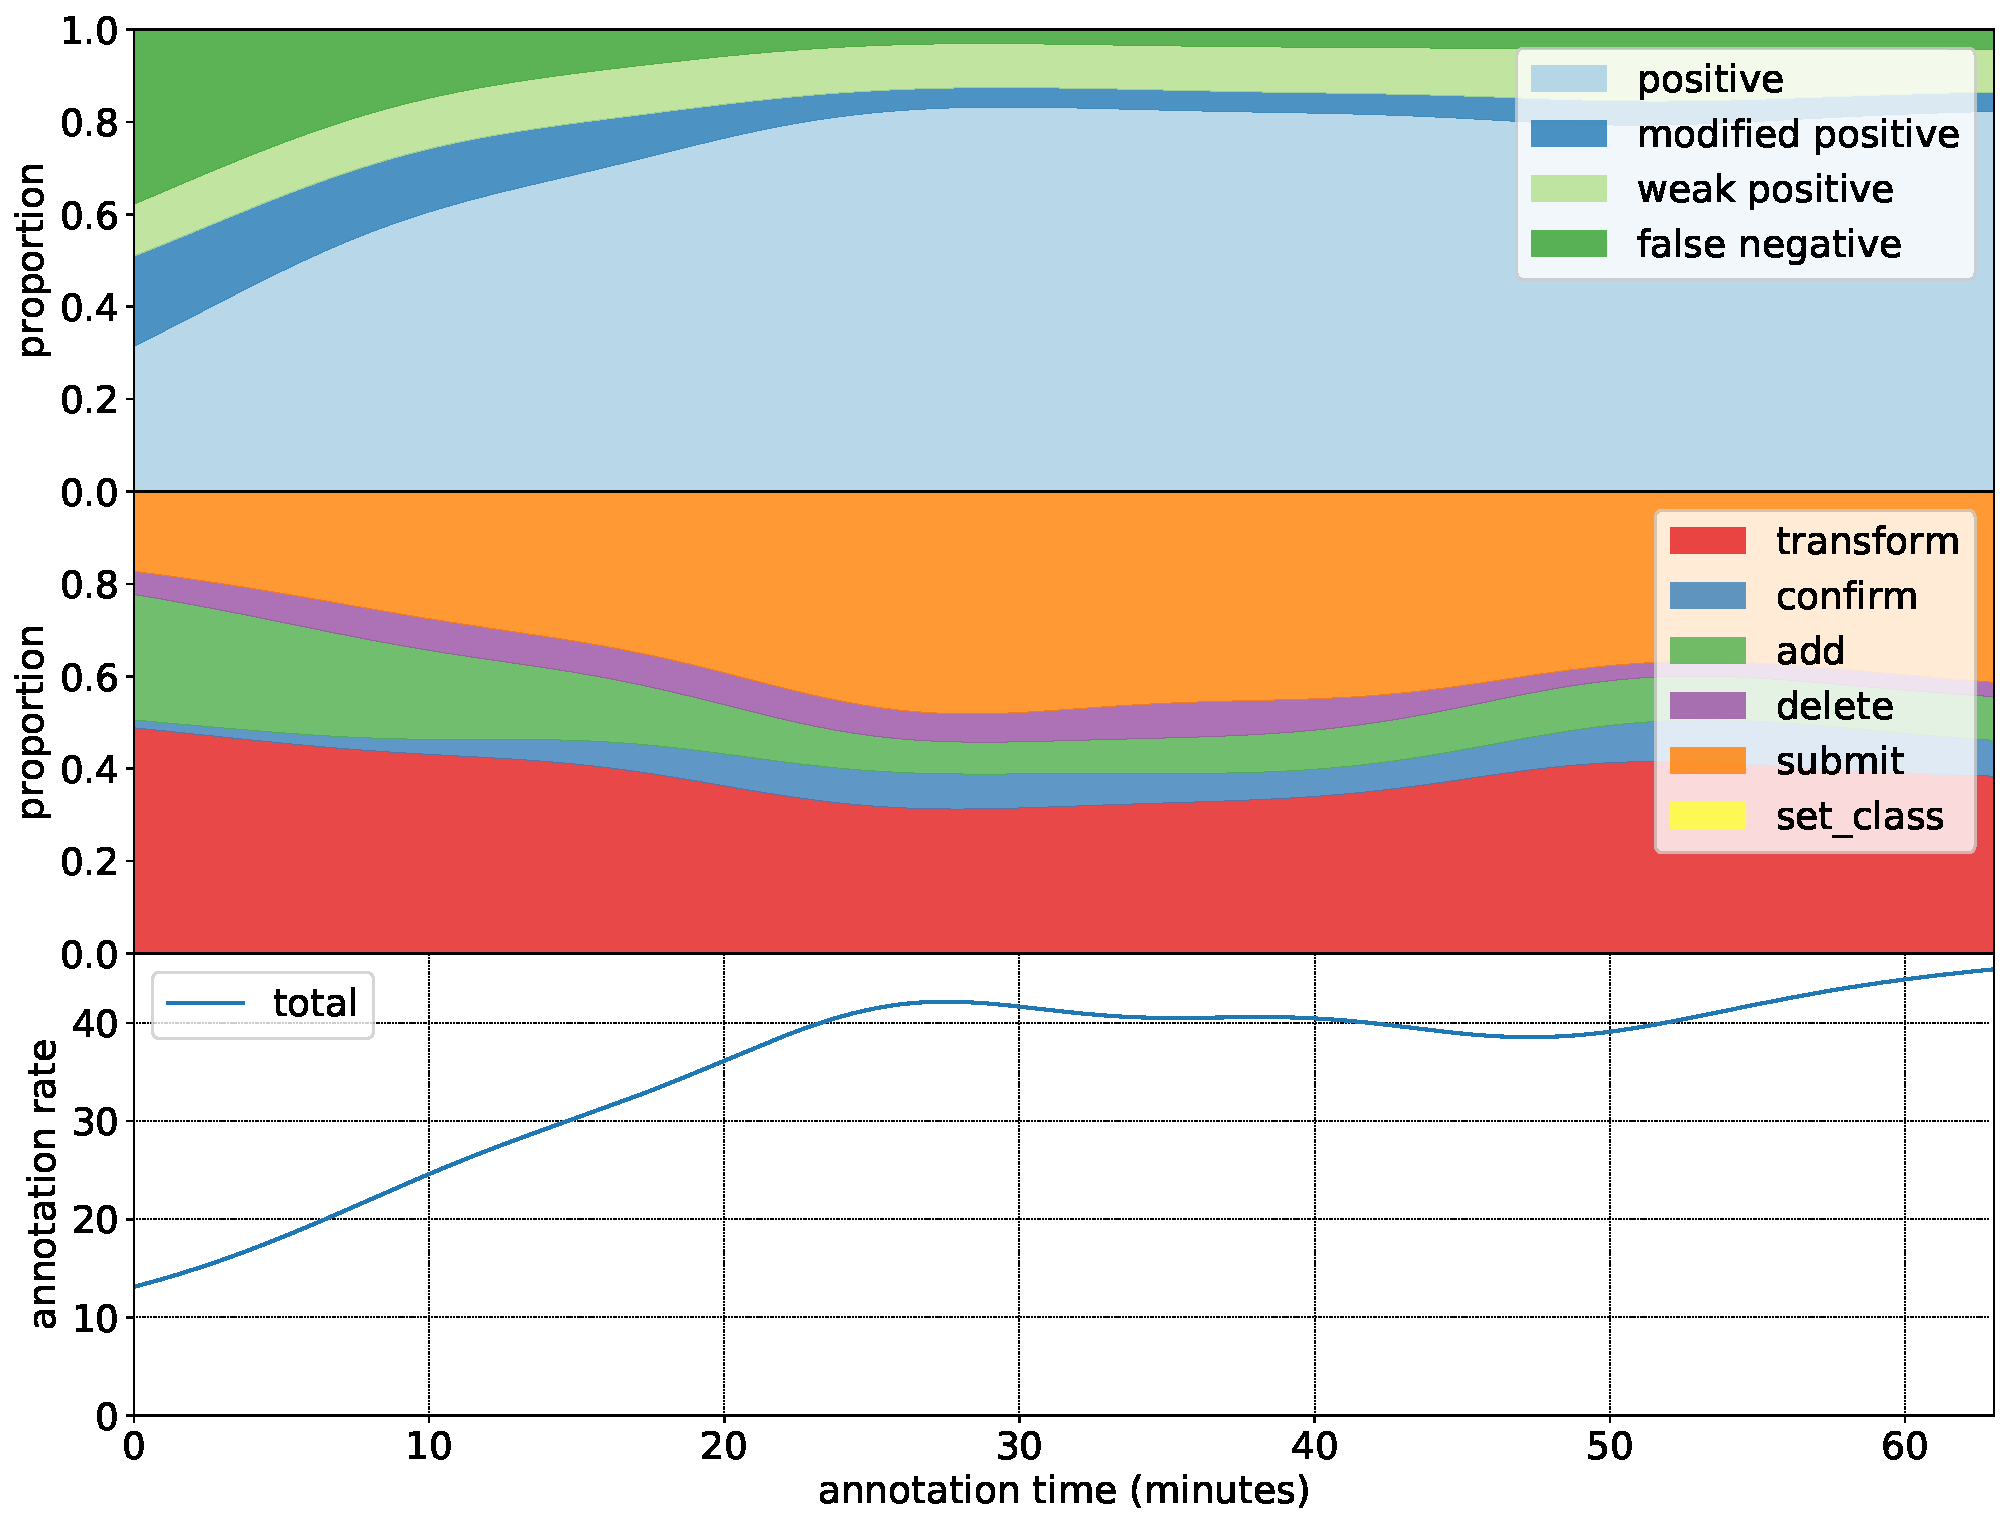
\includegraphics[width=1.0\linewidth]{charts/action_annotations/branches.pdf}
\caption{  }
\label{fig:branches_annotation}
\end{figure}

\pagebreak
\section {scallop}

\begin{figure*}[!h]
  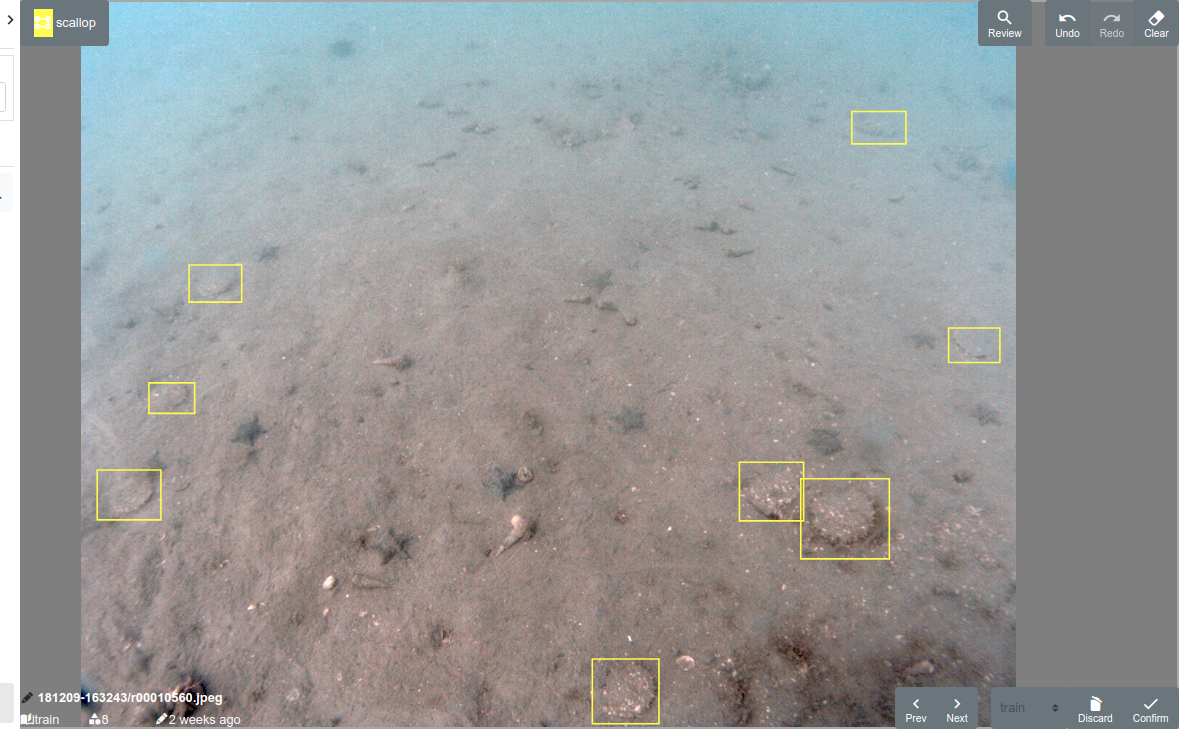
\includegraphics[width=0.475\linewidth]{figures/annotation/screenshots/scallops.png}
  \hfill
  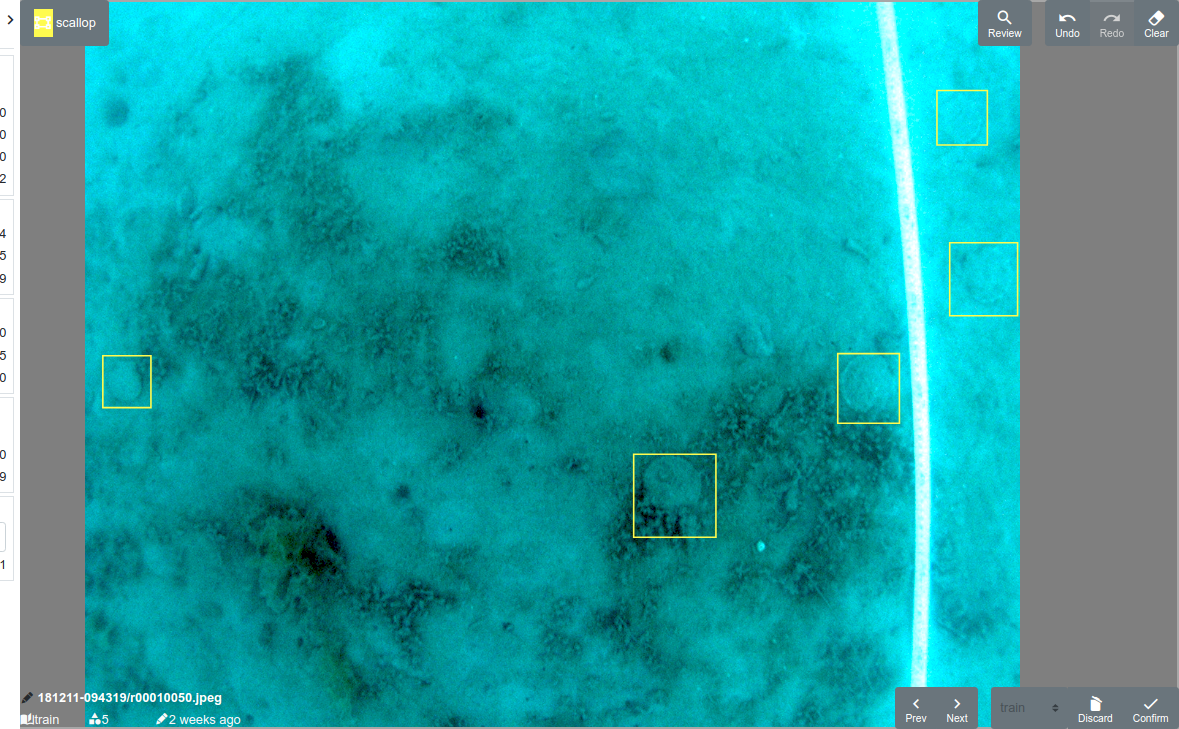
\includegraphics[width=0.475\linewidth]{figures/annotation/screenshots/scallops3.png}
\caption{Example images from the \emph{scallop} dataset}
\label{fig:scallop_dataset}  
\end{figure*}

\begin{figure}[!h]
\centering
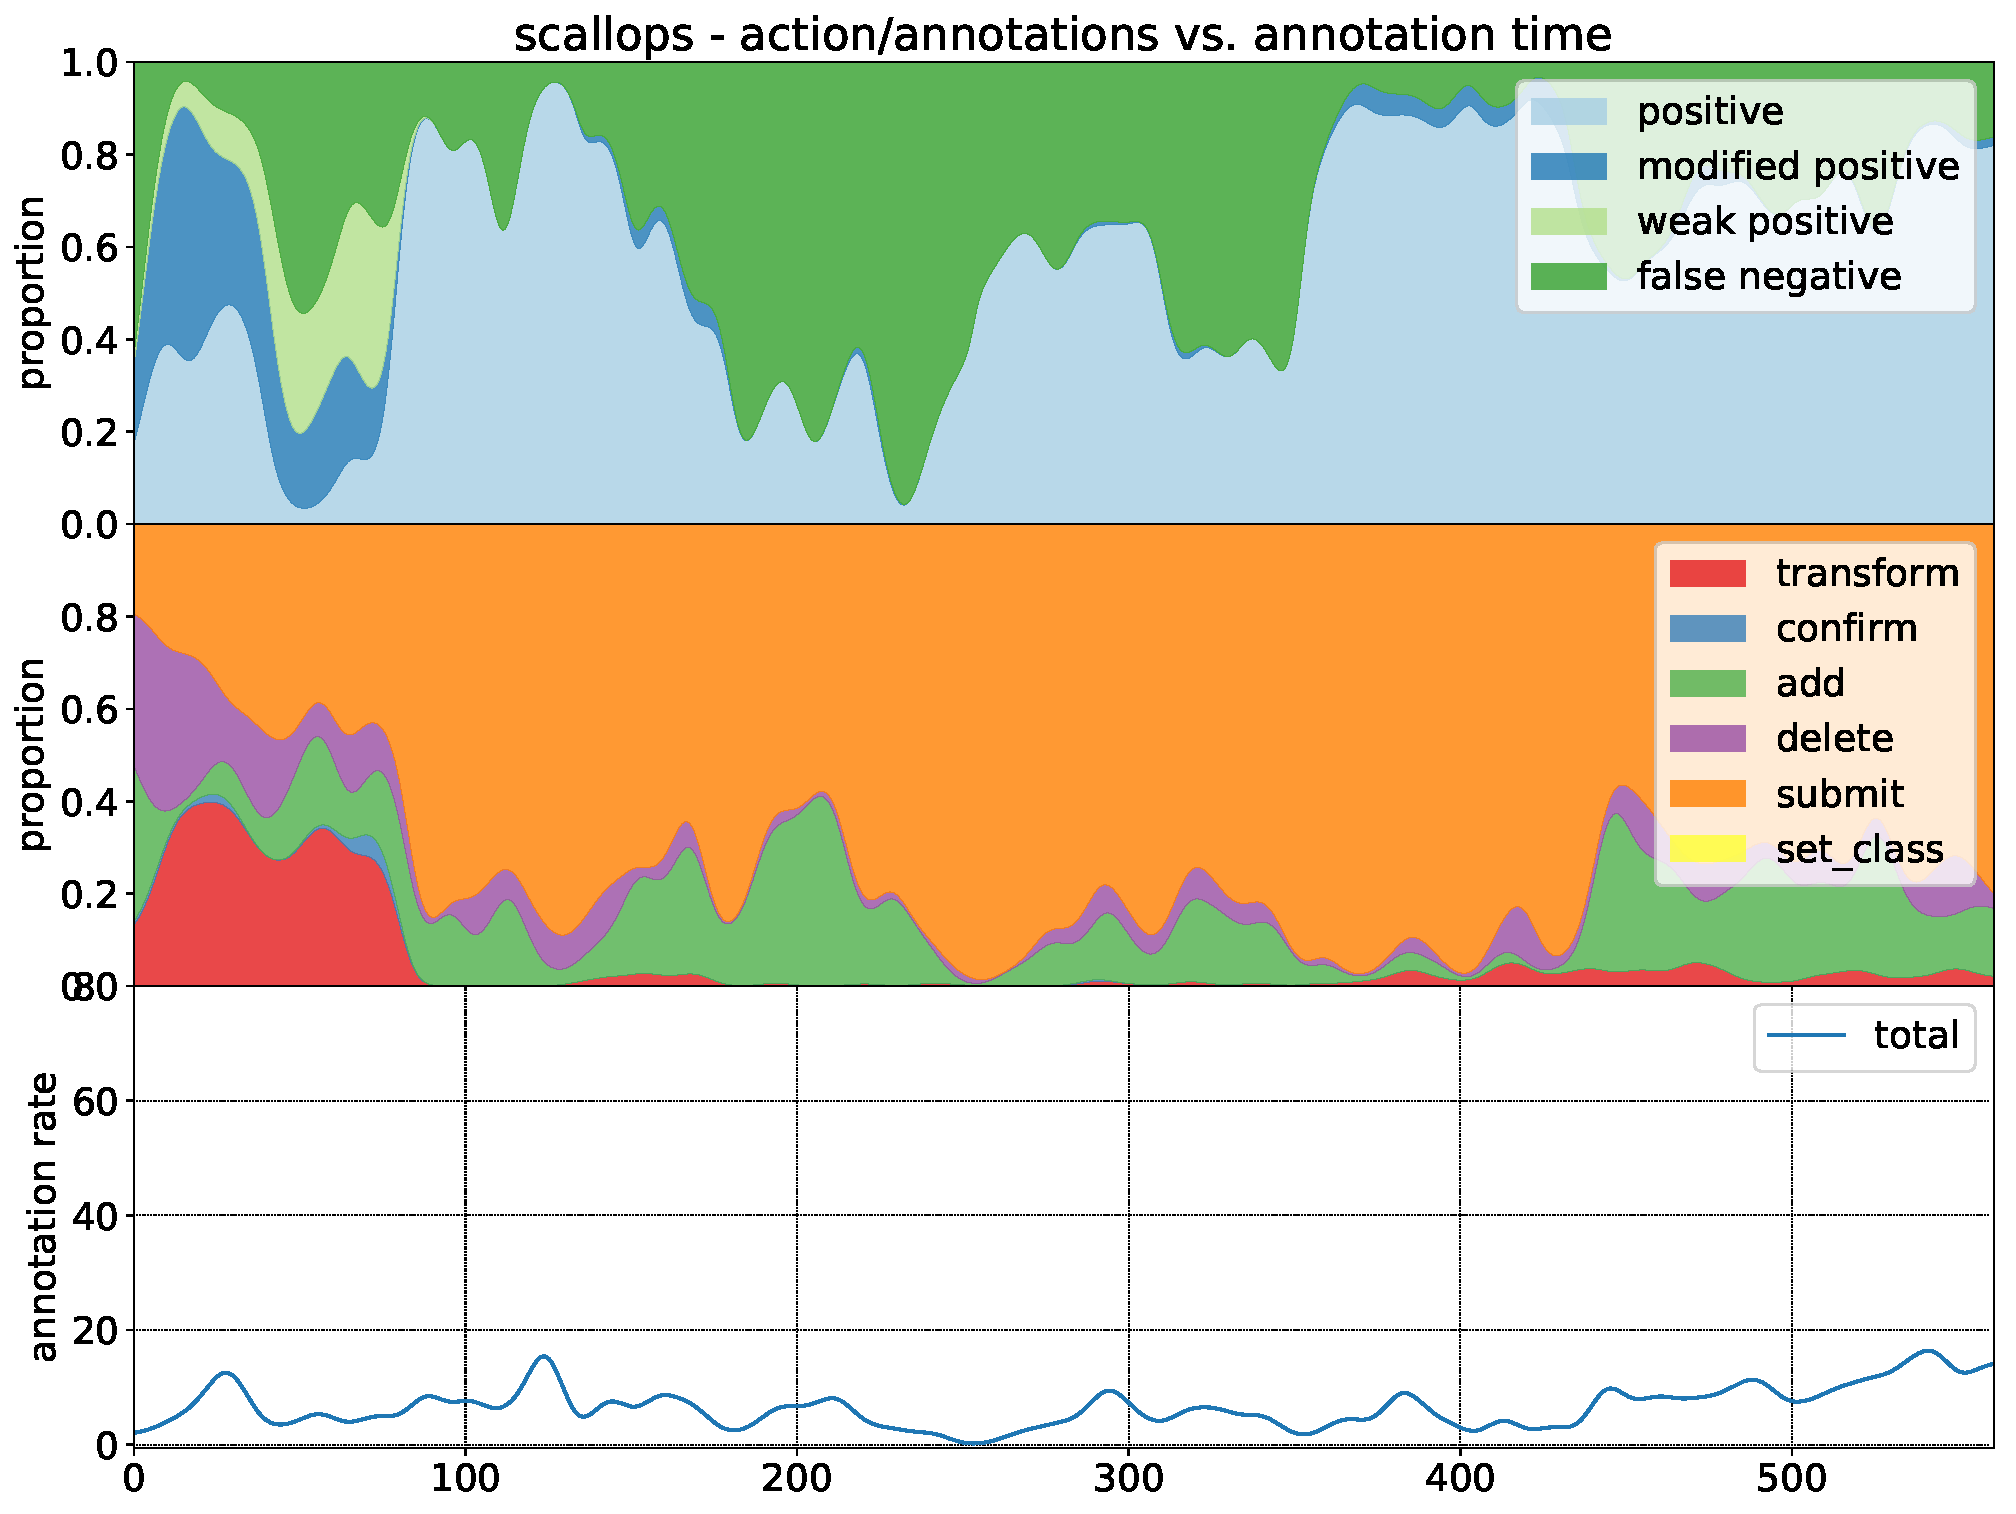
\includegraphics[width=1.0\linewidth]{charts/action_annotations/scallops.pdf}
\caption{  }
\label{fig:scallop_annotation}
\end{figure}

\pagebreak
\section {penguin survey}


\begin{figure*}[!h]
\centering
  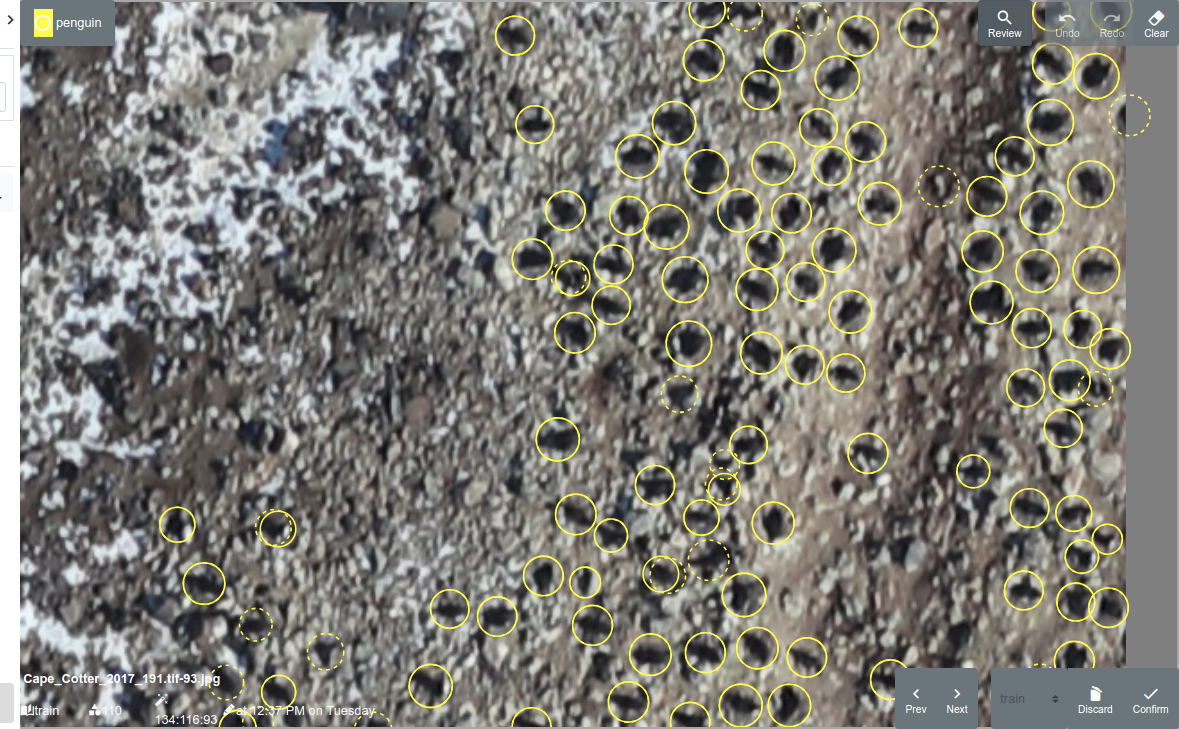
\includegraphics[width=0.475\linewidth]{figures/annotation/screenshots/penguins_aerial.png}
  \hfill
  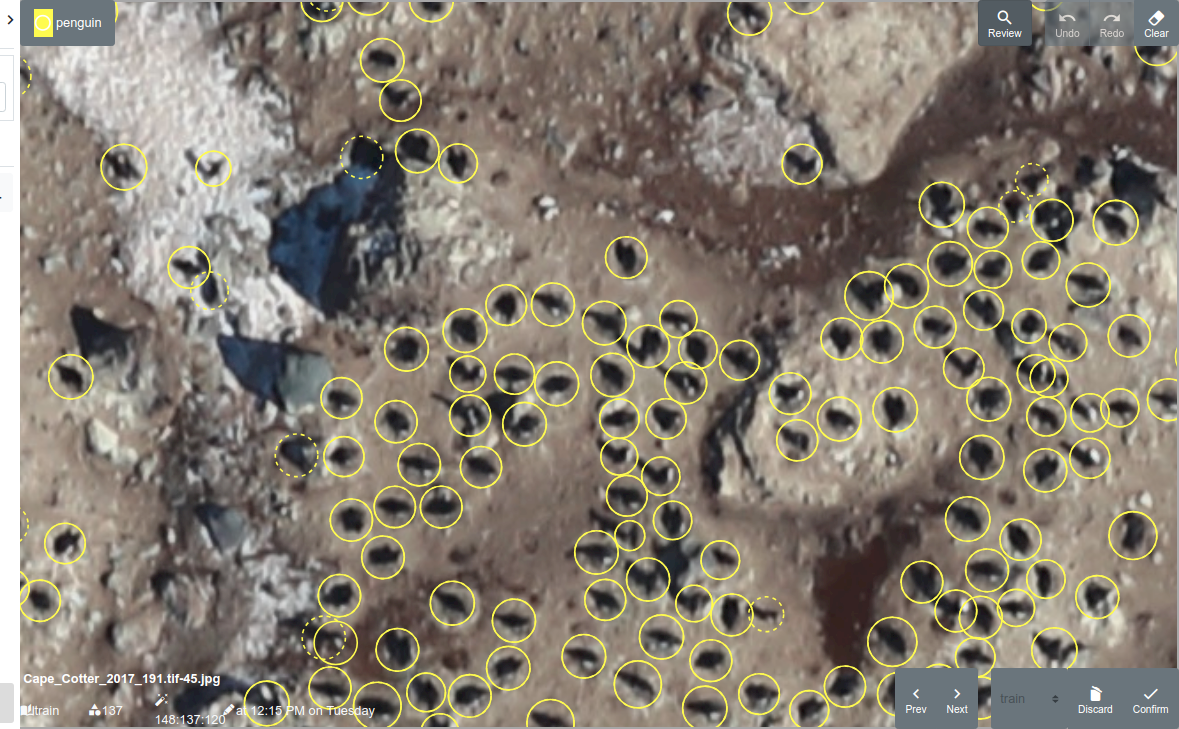
\includegraphics[width=0.475\linewidth]{figures/annotation/screenshots/penguins_aerial2.png}
  \caption{}
\caption{ Example images from the \emph{penguin survey} dataset}
\label {fig:penguin_aerial_examples}
\end{figure*}

\begin{figure}[!h]
\centering
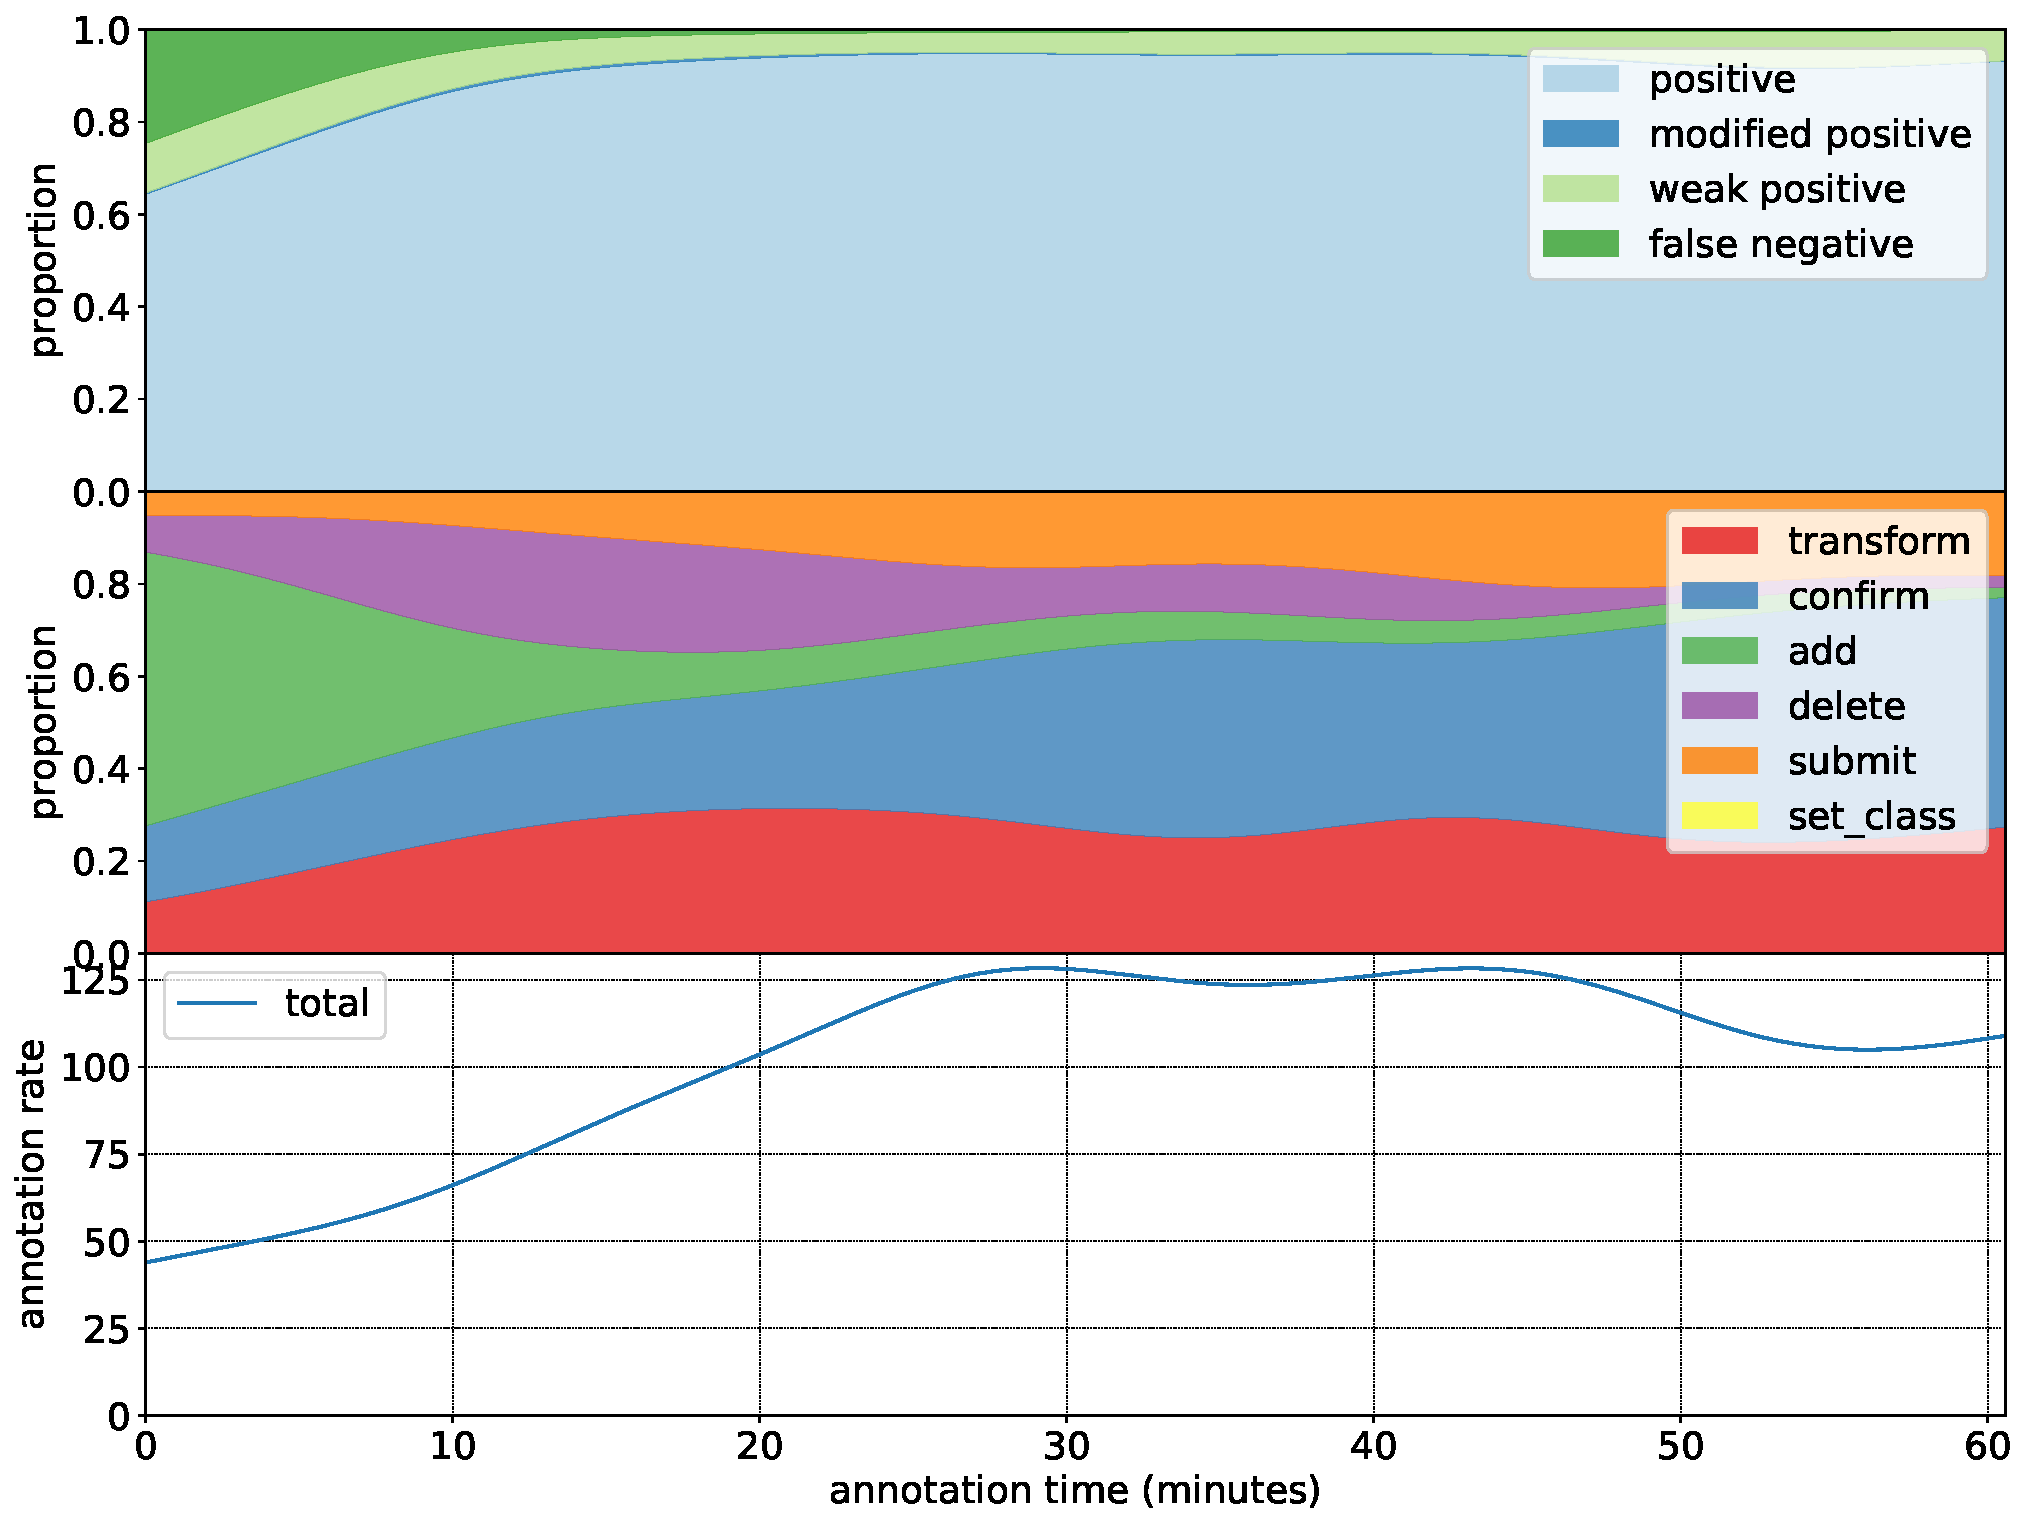
\includegraphics[width=1.0\linewidth]{charts/aerial_penguins/action_annotations/cotter_a.pdf}
\caption{  }
\label{fig:cotter_annotation}
\end{figure}

\pagebreak
\begin{figure}[H]
\begin{minipage}[c][\textheight]{\textwidth}
\centering
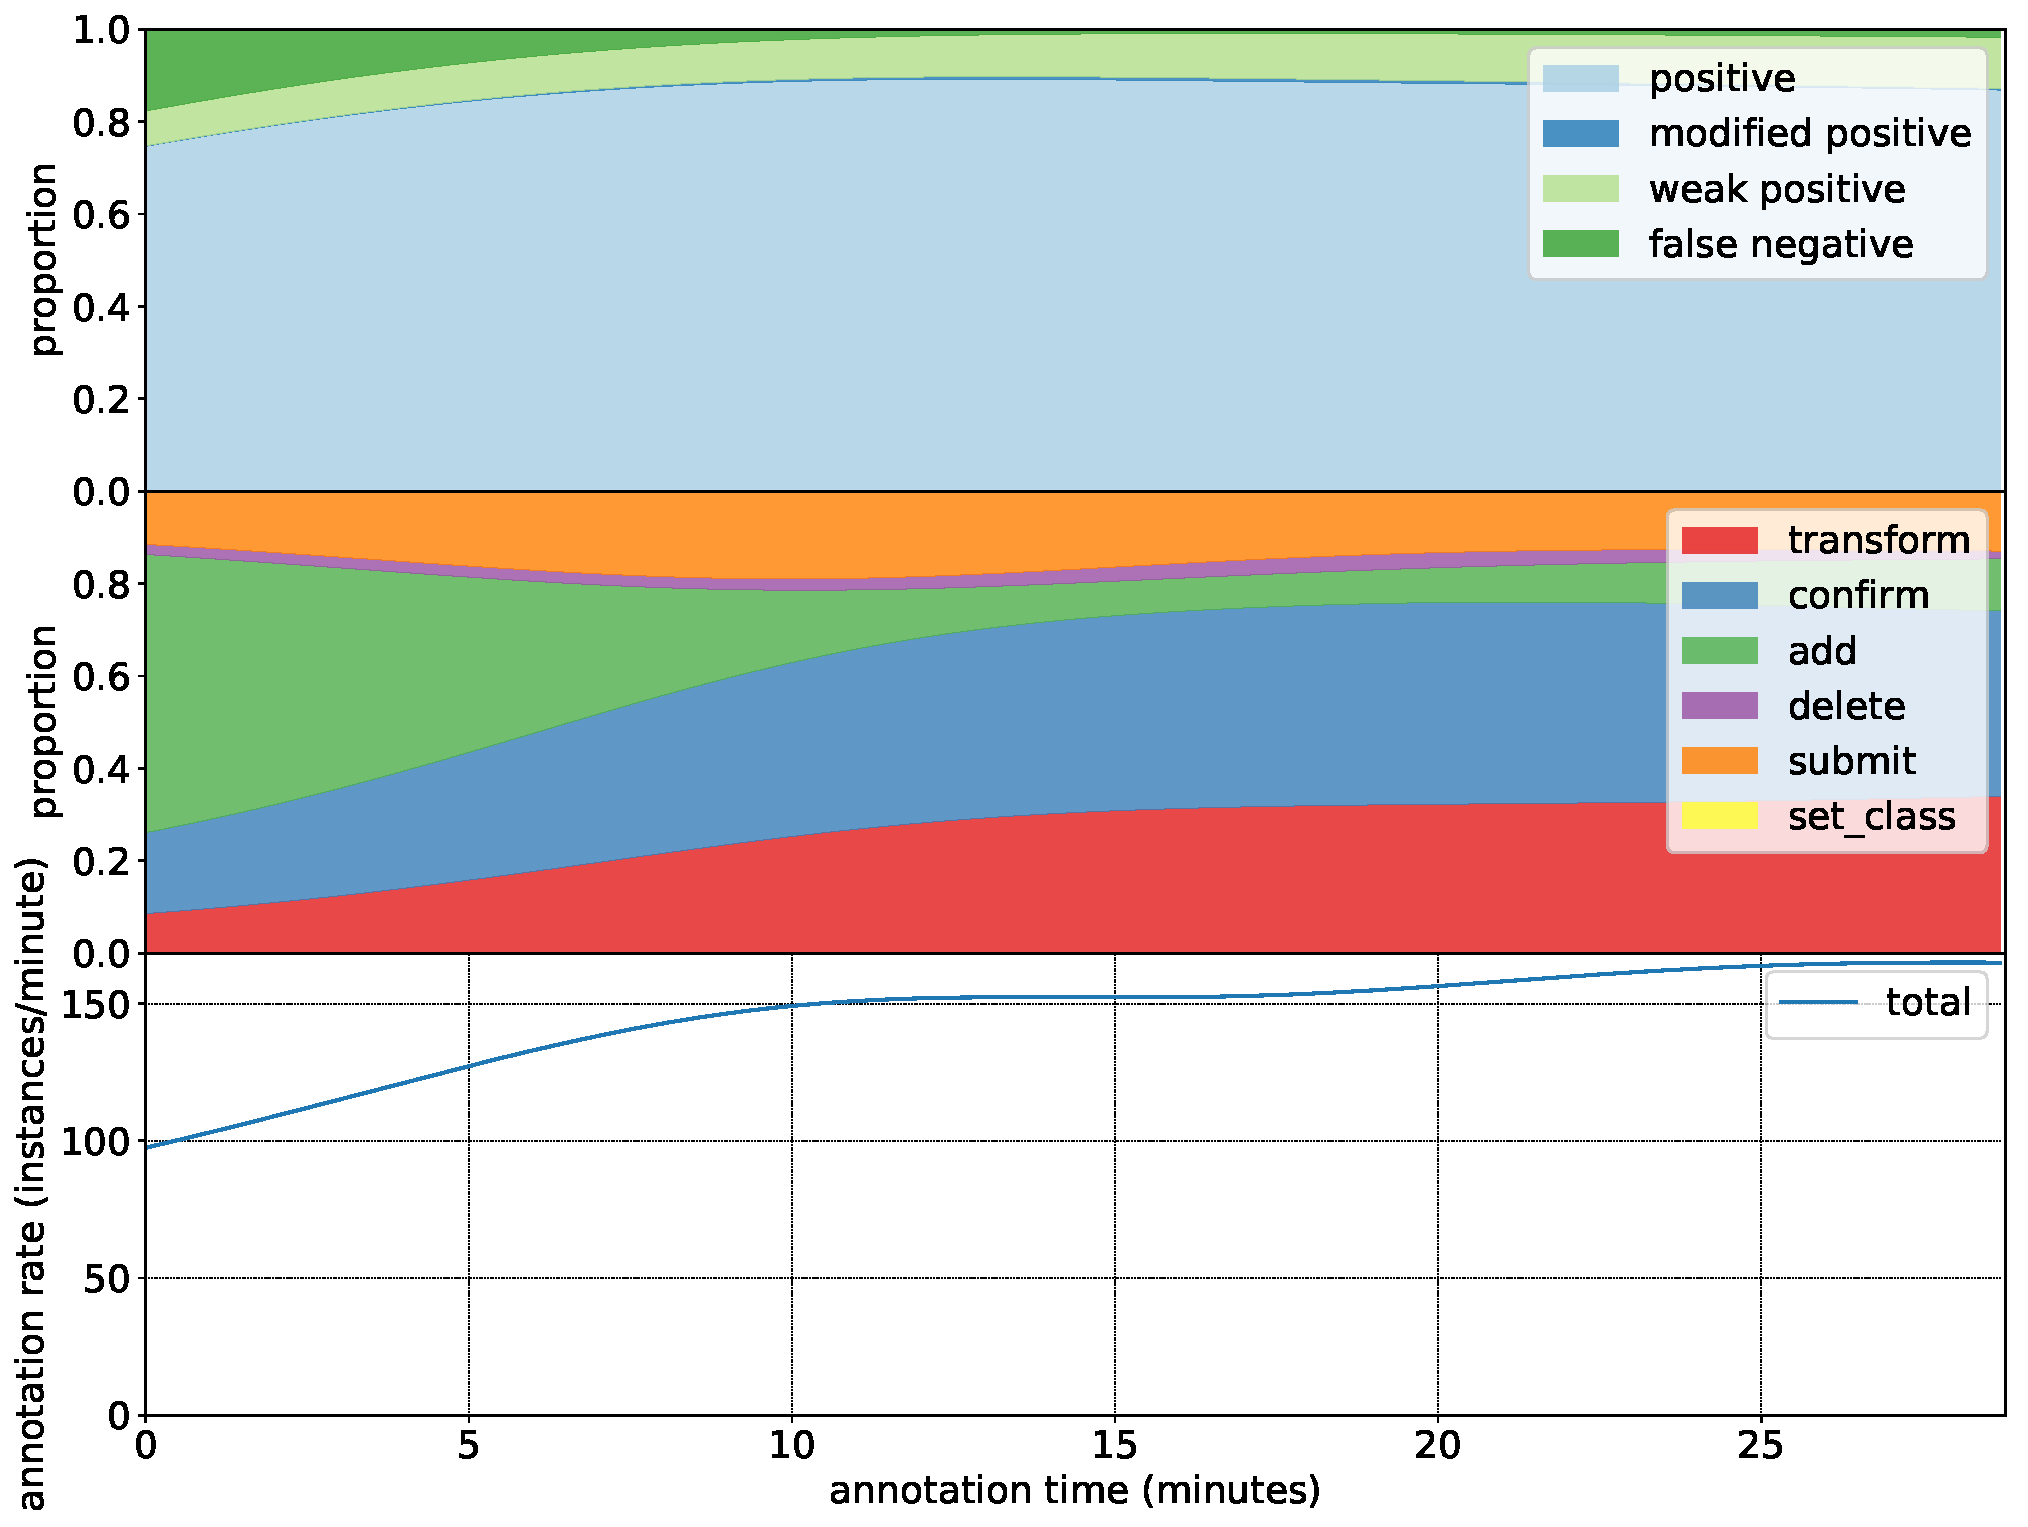
\includegraphics[width=1.0\linewidth]{charts/aerial_penguins/action_annotations/hallett_a.pdf}
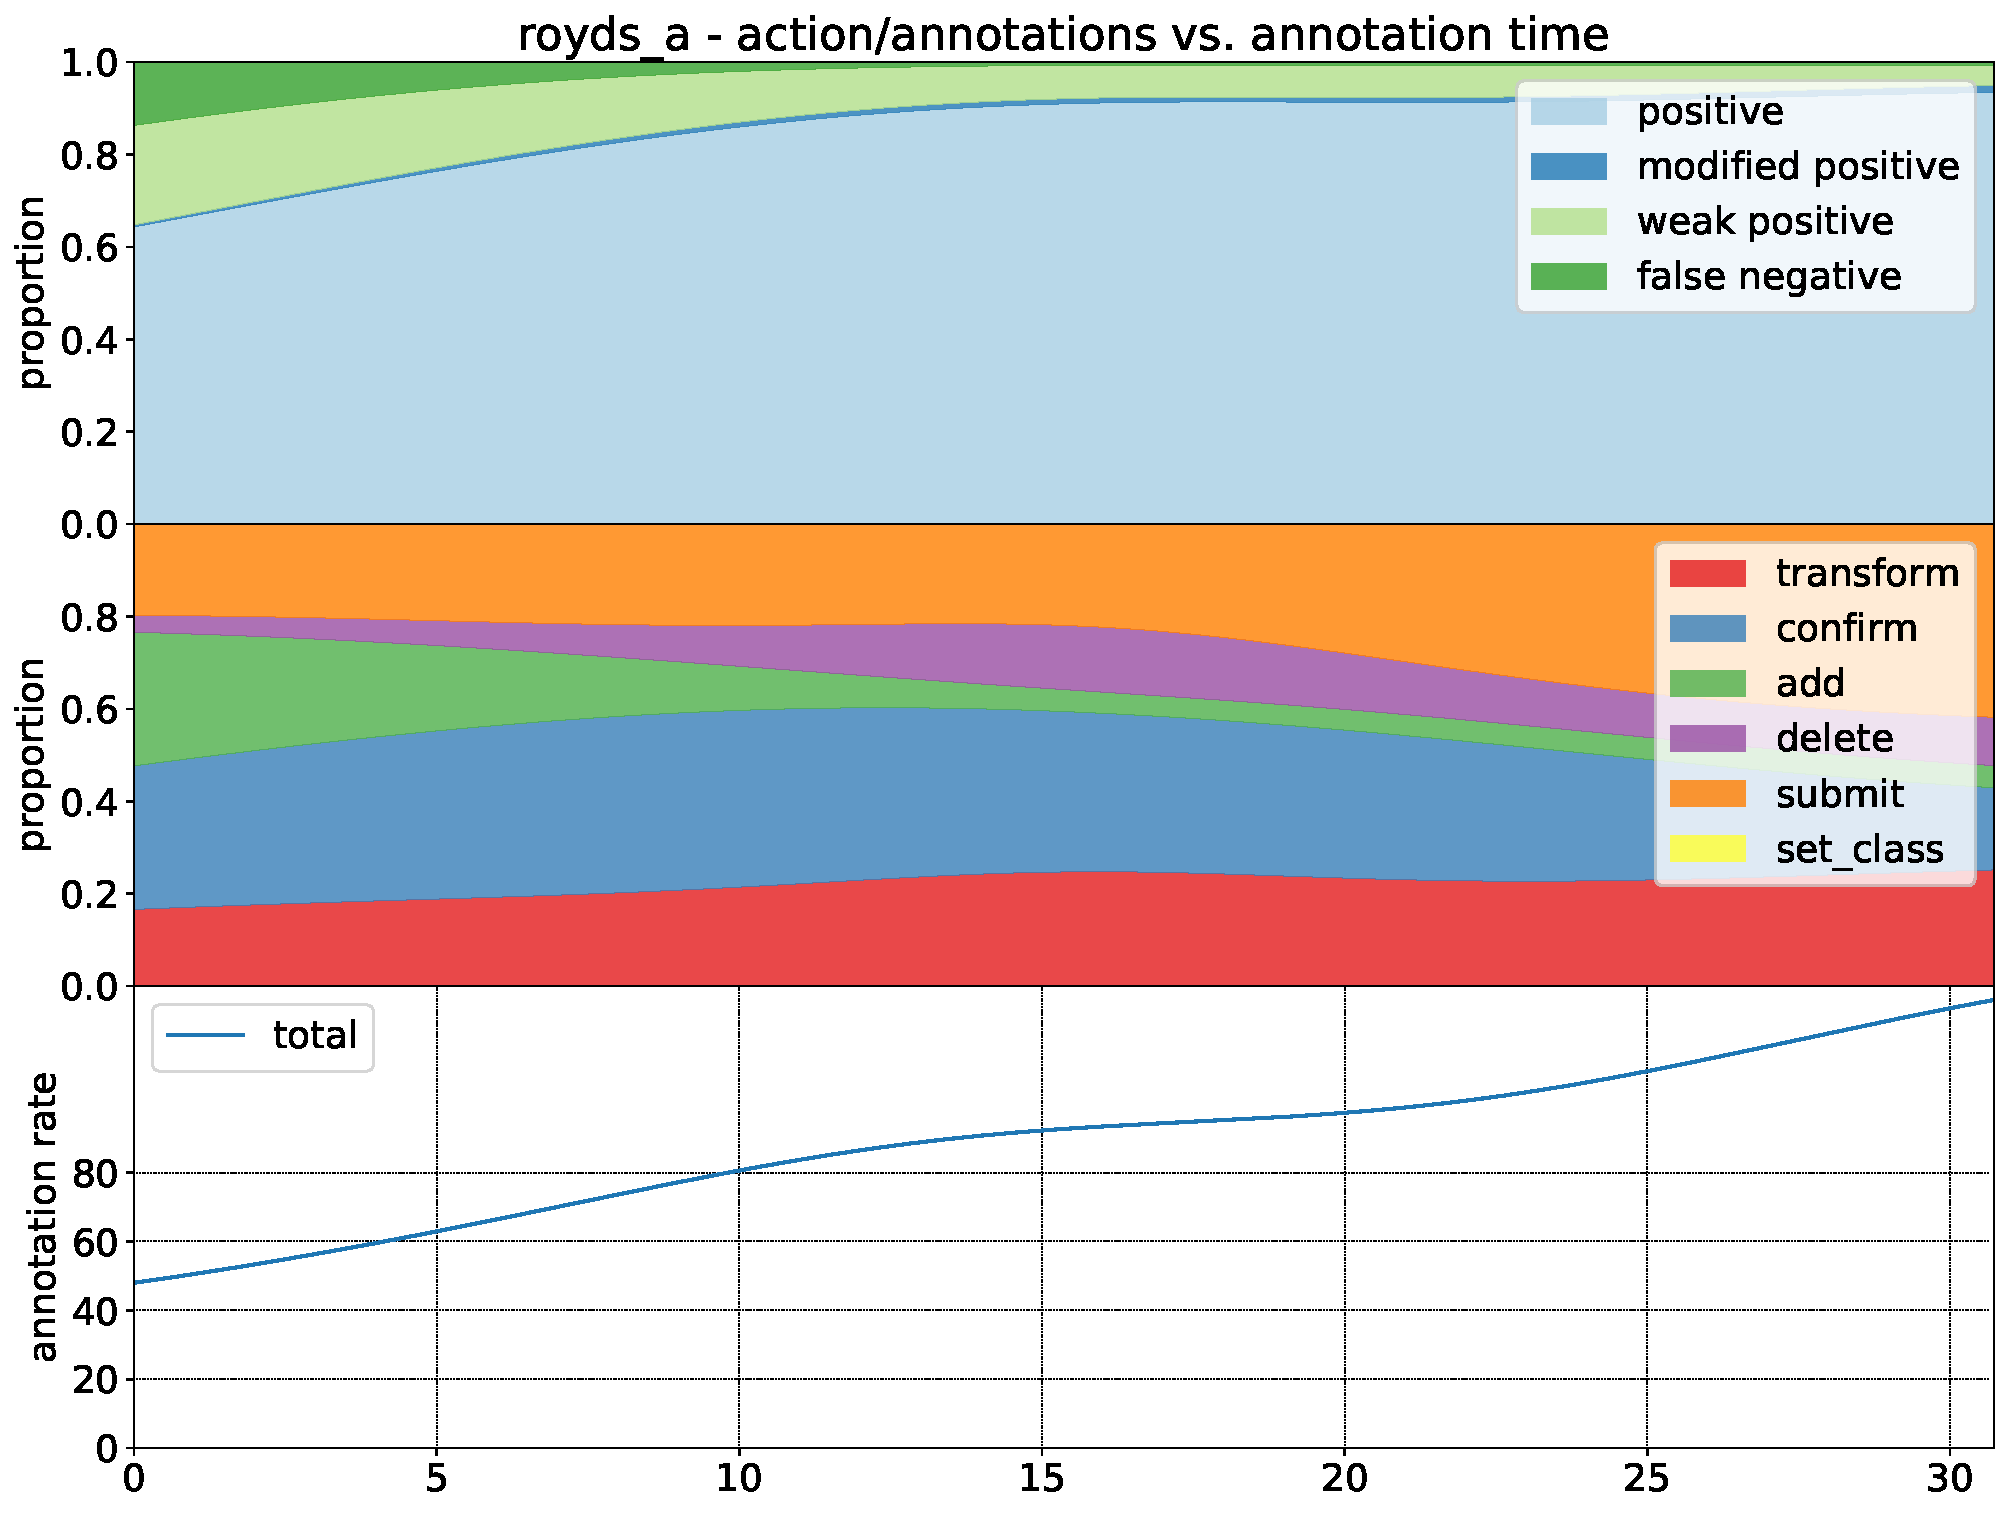
\includegraphics[width=1.0\linewidth]{charts/aerial_penguins/action_annotations/royds_a.pdf}
\caption{  }
\label{fig:royds_annotation}
\end{minipage}
\end{figure}


\pagebreak
\section {seals}

\begin{figure*}[!h]
\centering
  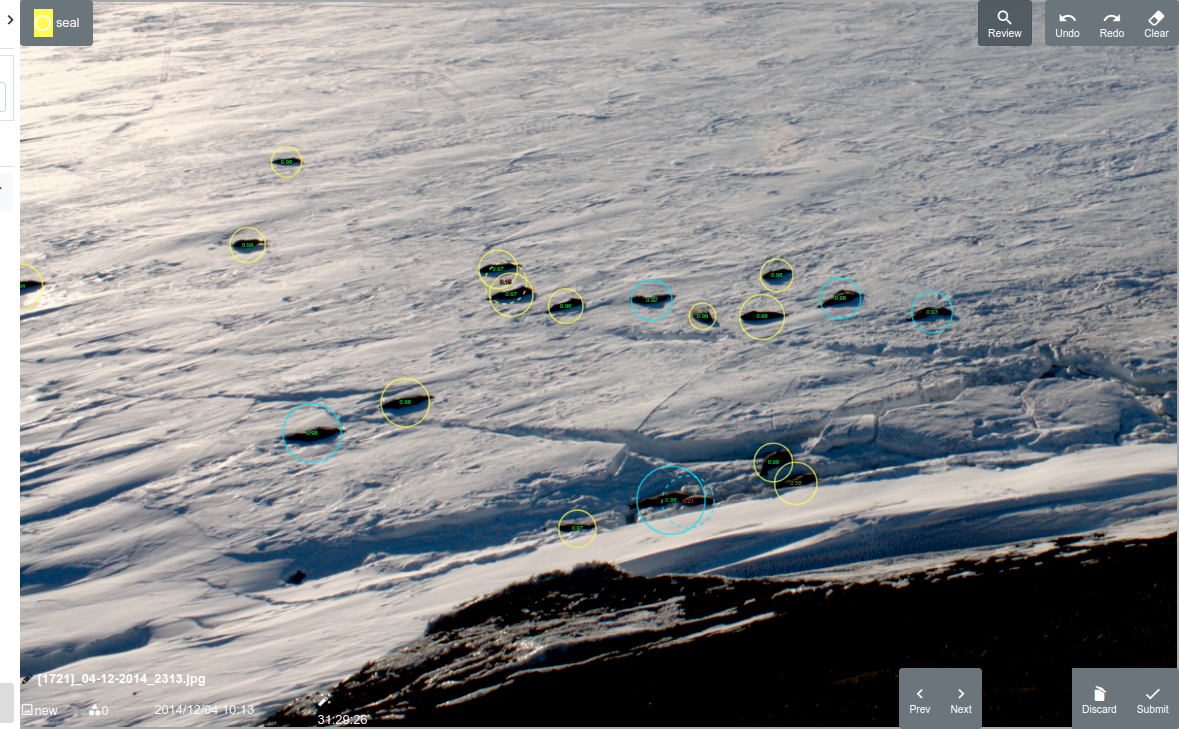
\includegraphics[width=0.475\linewidth]{figures/annotation/screenshots/seals_small2.png}
  \hfill
  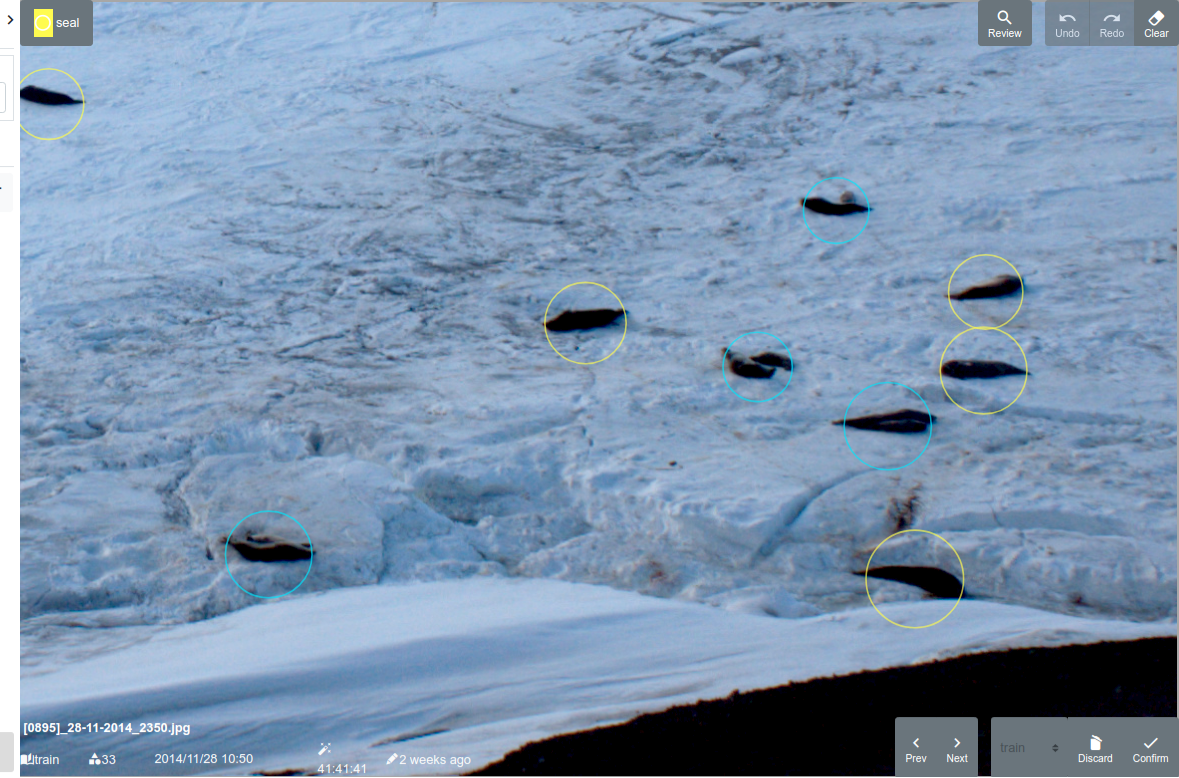
\includegraphics[width=0.45\linewidth]{figures/annotation/screenshots/seals_big.png}
  \caption{}
\caption{ Example images from the \emph{seals} dataset}
\label {fig:seals_examples}
\end{figure*}

\begin{figure}[!h]
\centering
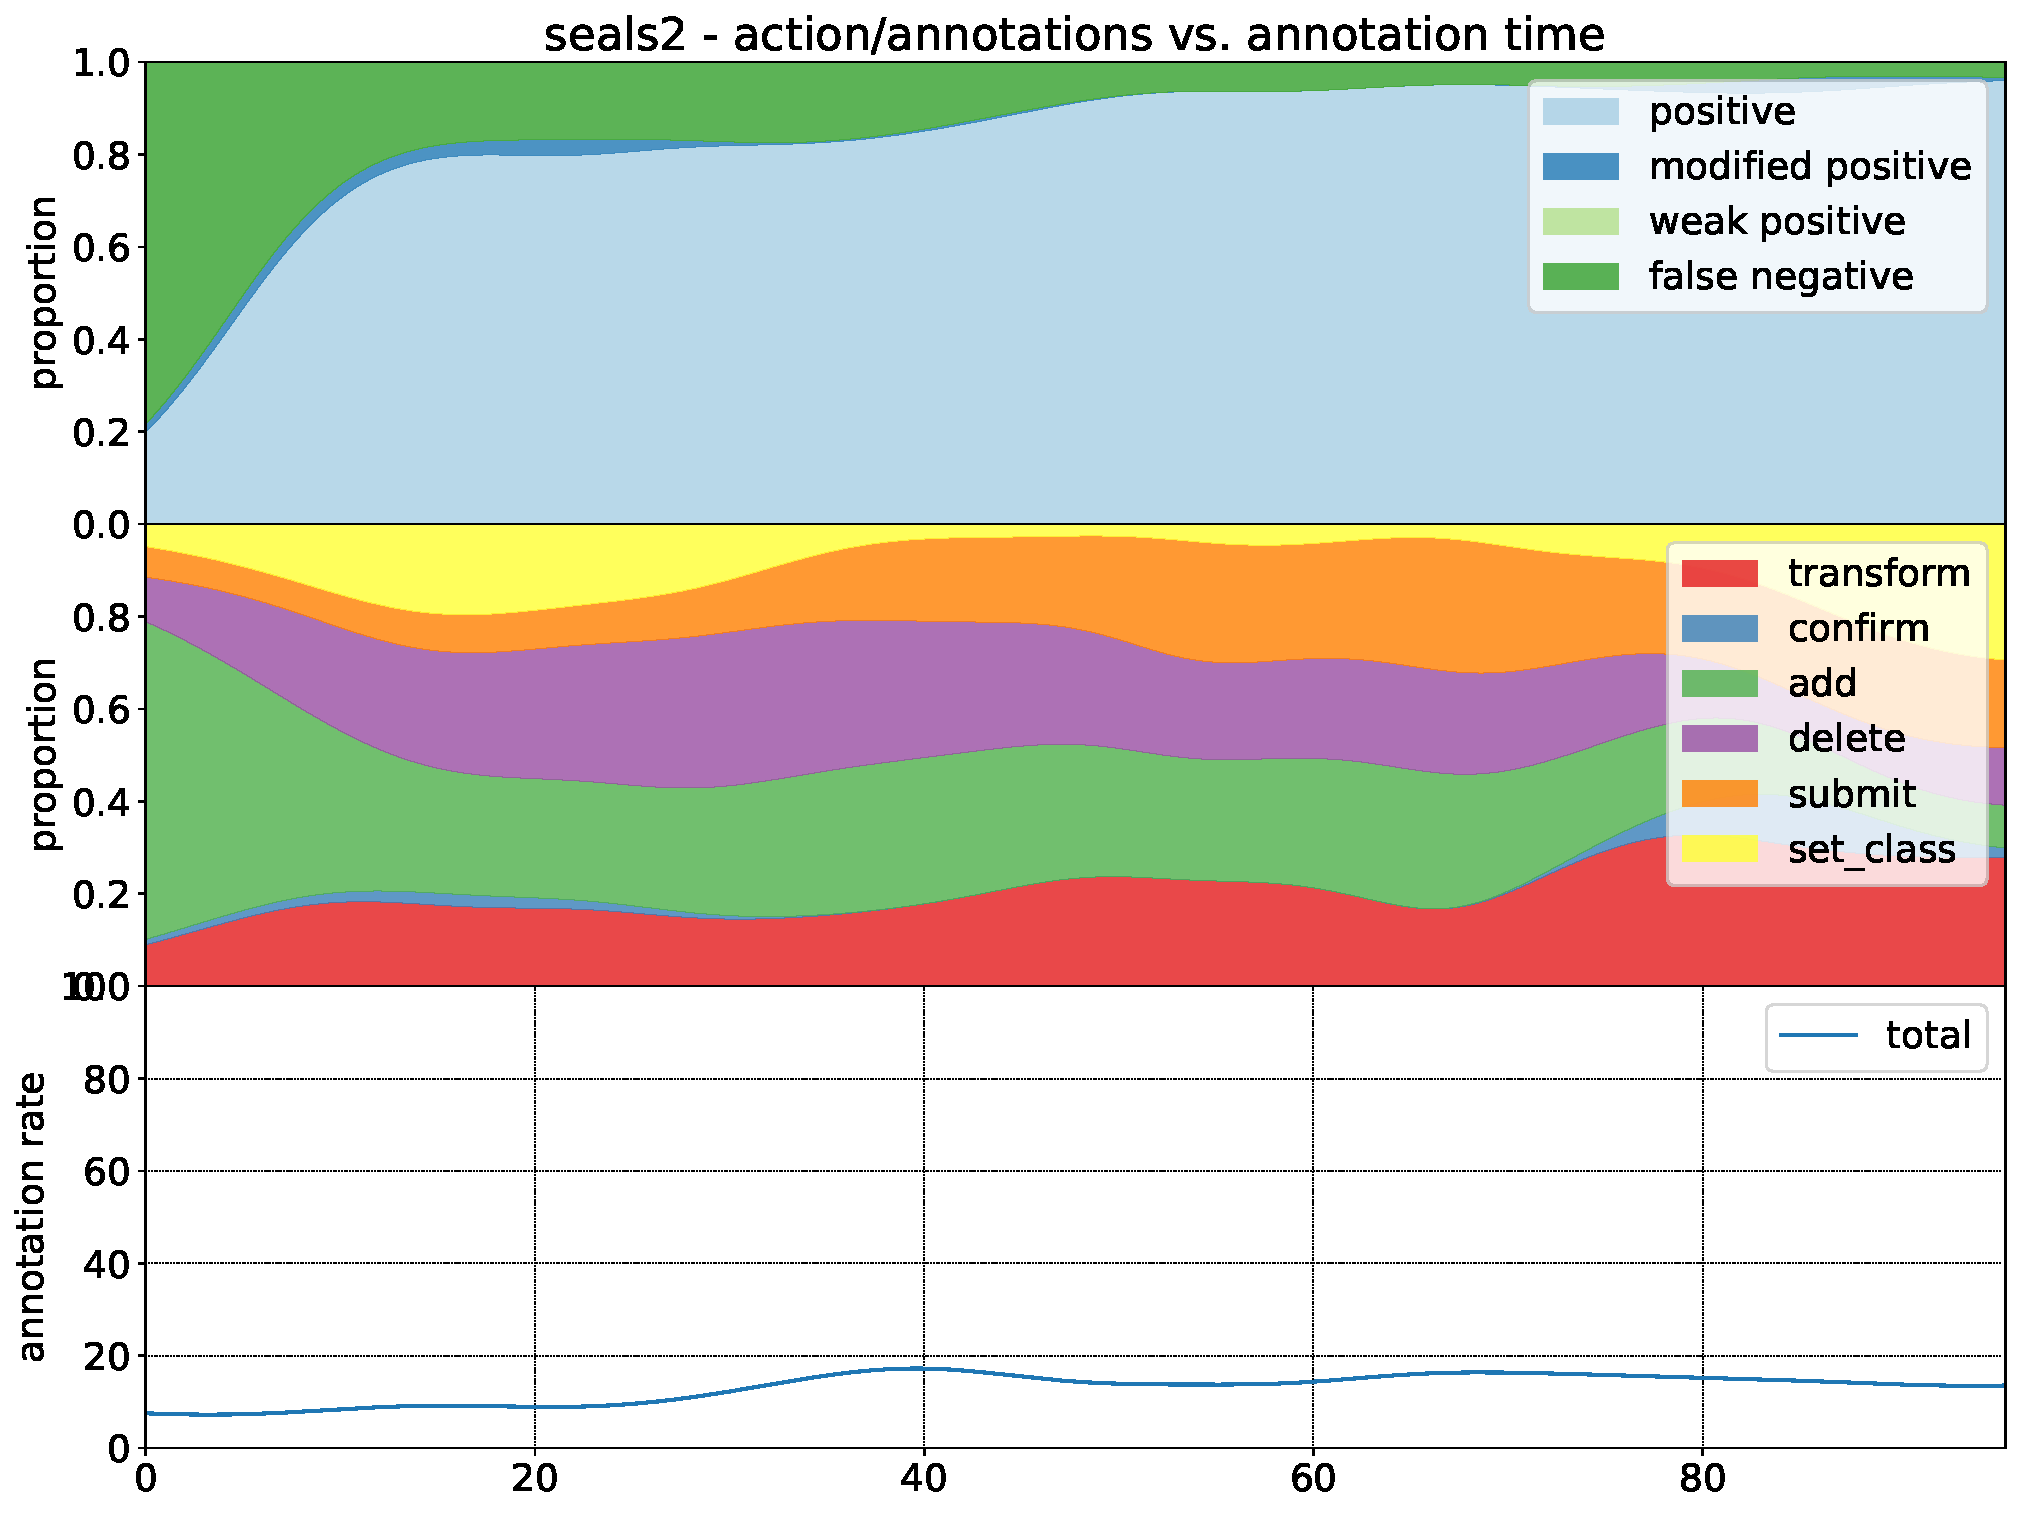
\includegraphics[width=1.0\linewidth]{charts/action_annotations/seals2.pdf}
\caption{  }
\label{fig:seals2_annotation}
\end{figure}


\pagebreak
\section {scott base}

\begin{figure*}[!h]
\centering
  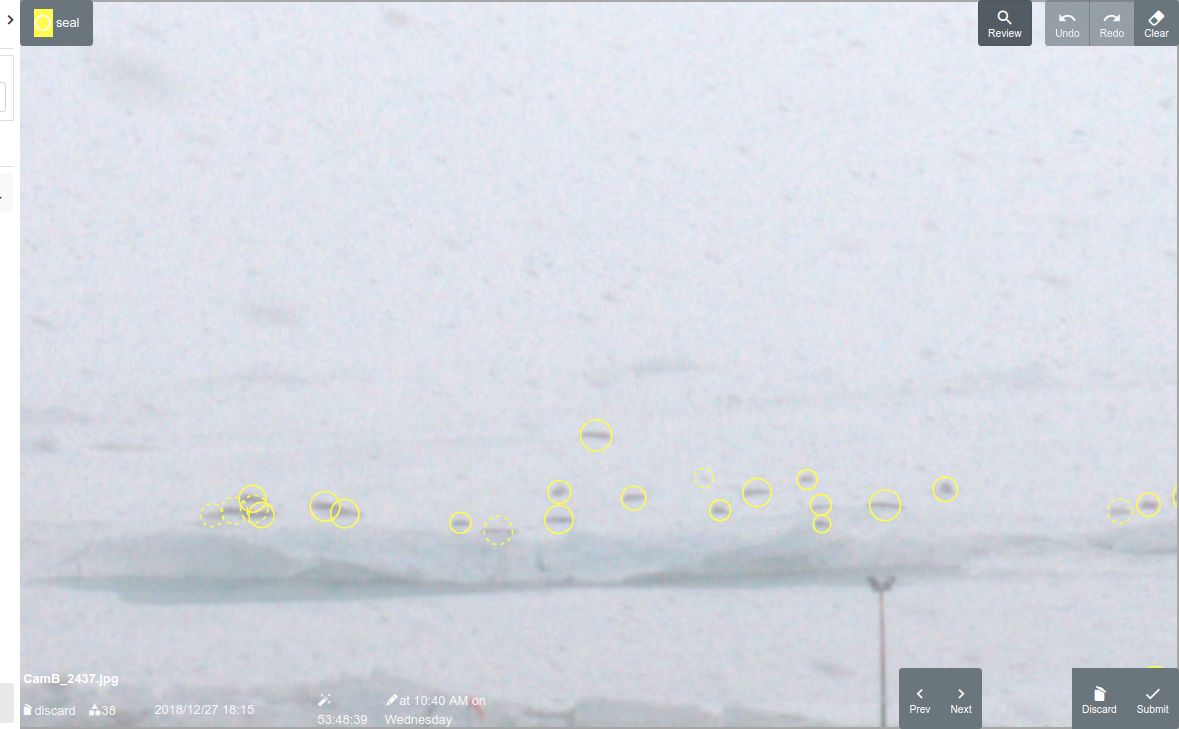
\includegraphics[width=0.475\linewidth]{figures/annotation/screenshots/scott_base_storm.png}
  \hfill
  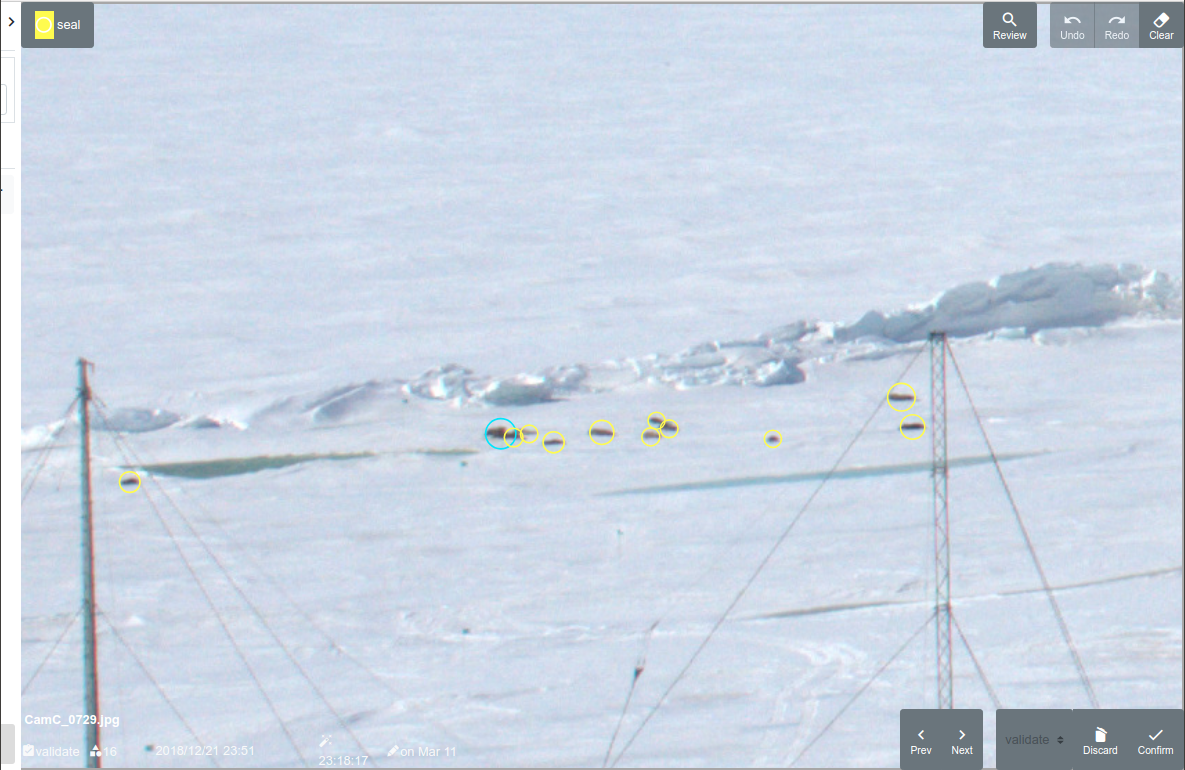
\includegraphics[width=0.45\linewidth]{figures/annotation/screenshots/scott_base_sunny.png}
  \caption{}
\caption{ Example images from the \emph{scott base} dataset}
\label {fig:scott_base_examples}
\end{figure*}

\begin{figure}[!h]
\centering
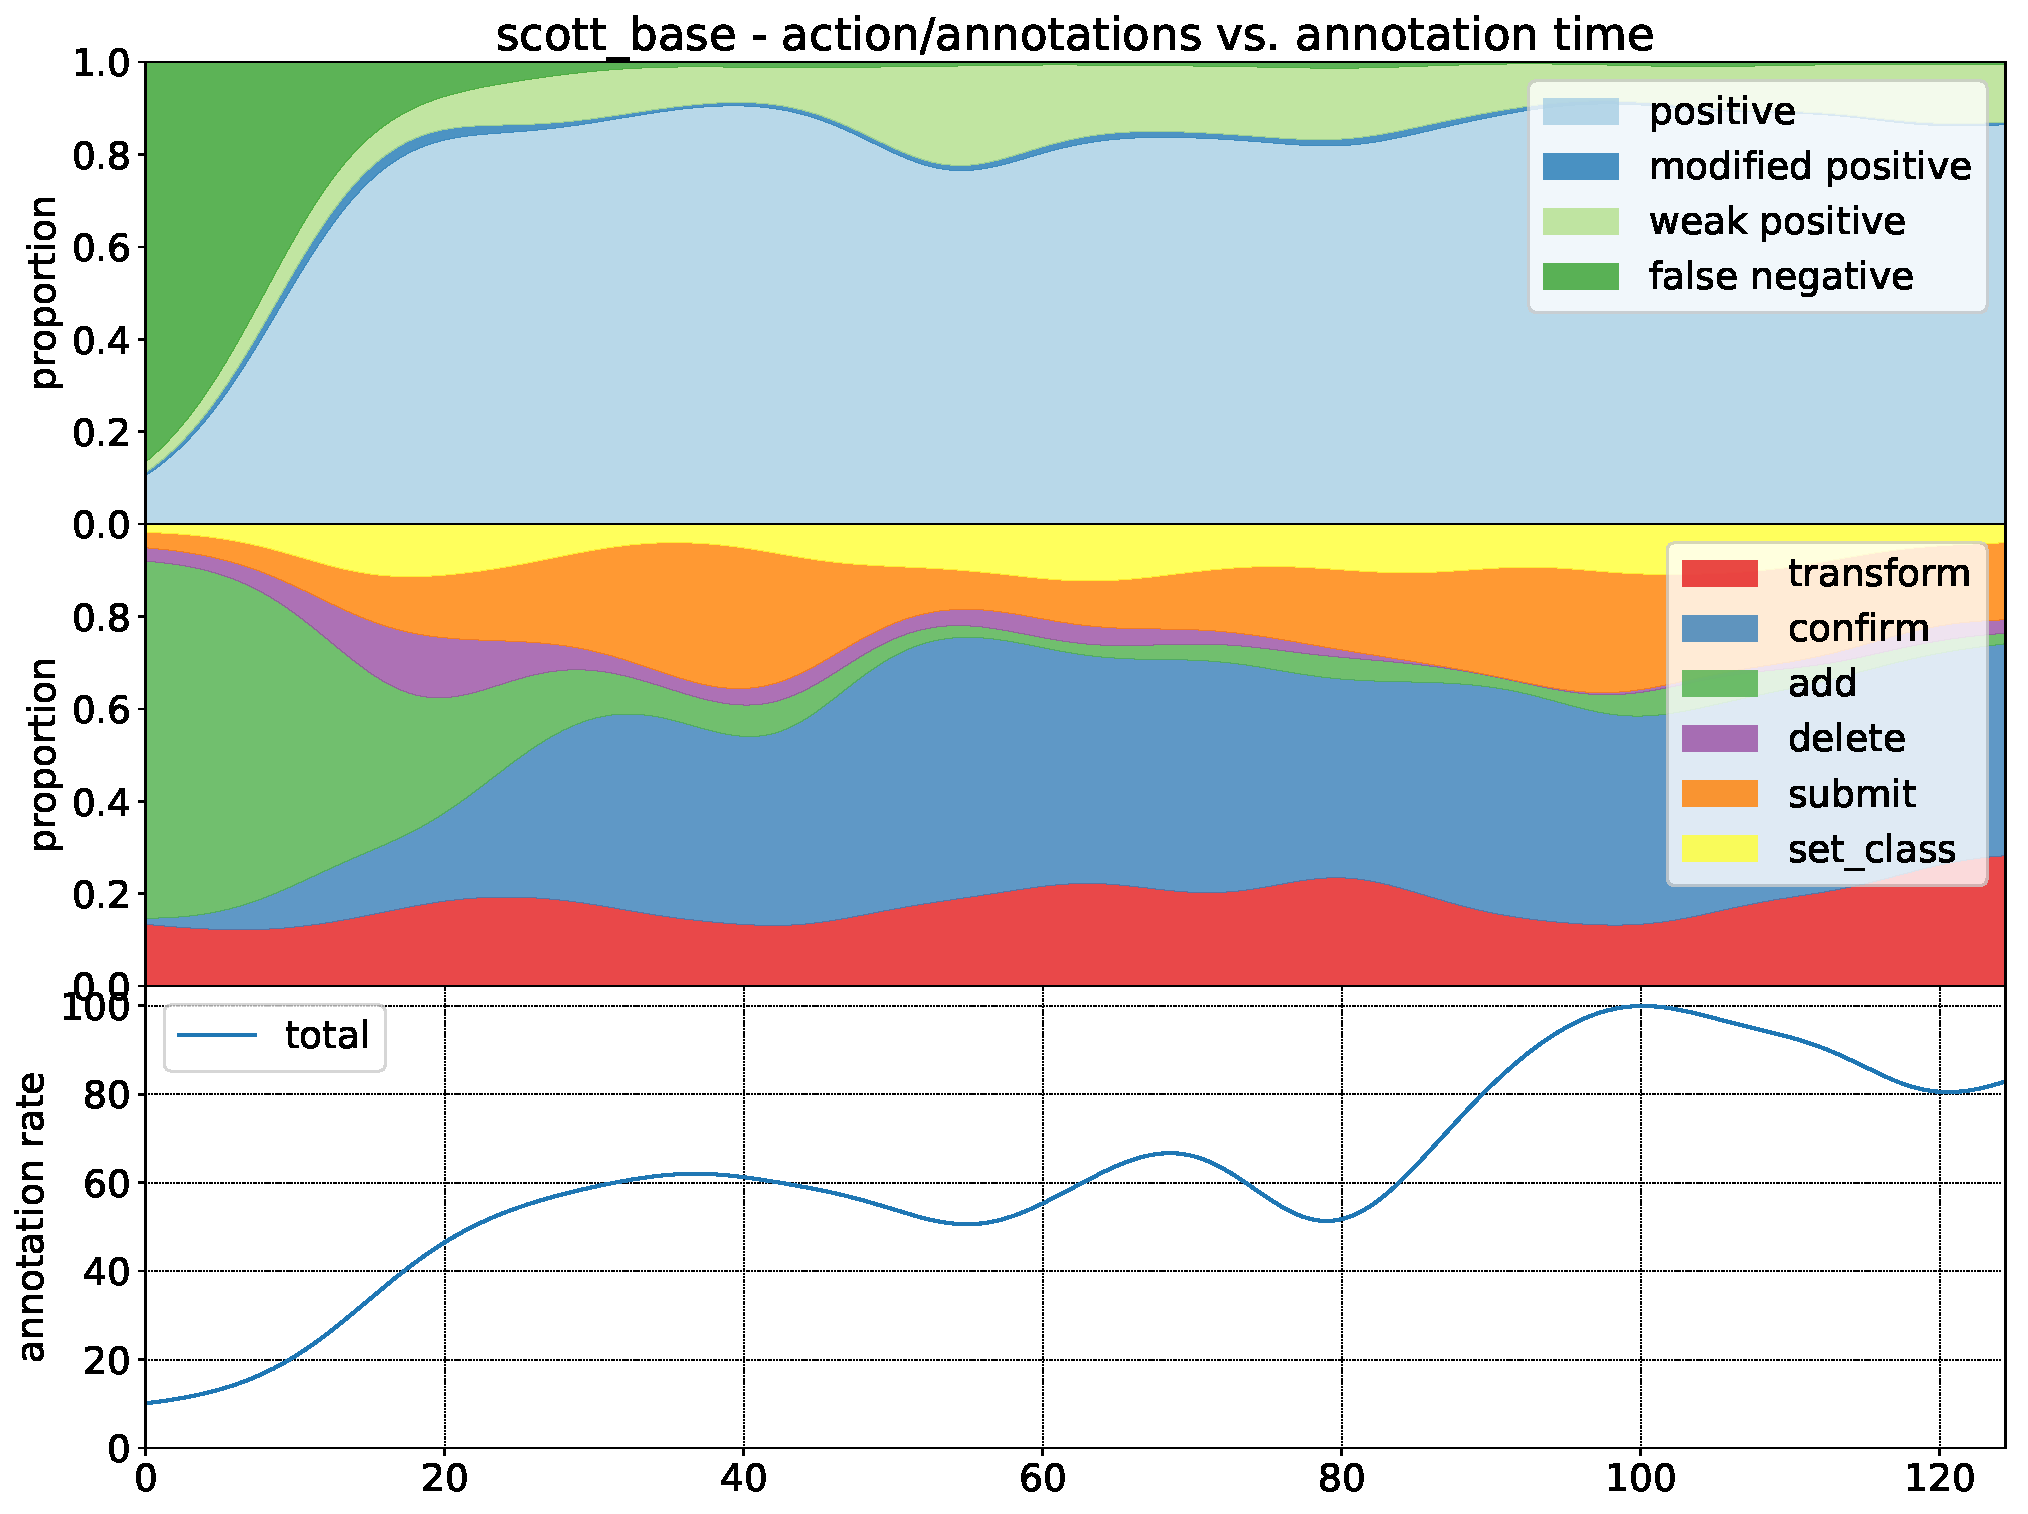
\includegraphics[width=1.0\linewidth]{charts/action_annotations/scott_base.pdf}
\caption{  }
\label{fig:scott_base_annotation}
\end{figure}